\documentclass[11pt,letterpaper]{article}
\usepackage[utf8]{inputenc}\usepackage[T1]{fontenc}\usepackage{lmodern}
\usepackage[spanish,es-noshorthands,es-tabla]{babel}\decimalpoint
\usepackage[margin=2.5cm]{geometry}\usepackage{booktabs,longtable,graphicx,amsmath,array,caption,xcolor,float,needspace}\usepackage[section]{placeins}\newcolumntype{L}[1]{>{\raggedright\arraybackslash}p{#1}}
\usepackage{upquote}
\usepackage[colorlinks=true,linkcolor=black,citecolor=black,urlcolor=blue]{hyperref}
\usepackage[round]{natbib}\captionsetup{font=small,labelfont=bf}
\setlength{\parskip}{4pt}
\begin{document}
\begin{center}{\Large\textbf{Envolvente de resistencia del desmonte ROM de Antamina con Leps 2.0}}\\[3pt]{\large Propuesta de curva e incertidumbre a alto confinamiento}\end{center}
\vspace{4pt}
\noindent\begin{tabular}{@{}p{3.2cm}p{12.6cm}@{}}\toprule
Para: & Compañía Minera Antamina\\
De: & Stantec\\
Fecha: & 12 de octubre de 2026\\\bottomrule
\end{tabular}

\section*{Resumen}
Stantec propone para el desmonte ROM de Antamina la curva de Leps 2.0
\begin{equation*}
\tau = \tan\!\left(48.47^{\circ} - 20^{\circ}\,e\right)\,(10p_a)^{0.15}\,\sigma_n'^{\,0.85},
\end{equation*}
donde $e$ es la relación de vacíos del desmonte colocado, con valor base 0.45. Con $e = 0.45$, el ángulo de fricción secante es 39.5° a 1~MPa, 33.3° a 4.62~MPa (el máximo ensayado en Antamina), 30.3° a 10~MPa y 28.8° a 15~MPa. La banda de incertidumbre de la curva va de 37.4° a 41.7° a 1~MPa y de 27.6° a 32.8° a 10~MPa.

La curva resulta de tres decisiones, cada una con su evidencia (sección~\ref{sec:decisiones}):
\begin{enumerate}
\item \textbf{El nivel sale de los ensayos de Antamina.} Los 37 ensayos (13 sets) de mármol, hornfels, intrusivo y mezclas dan $\phi'_{e=0} = 48.47^{\circ}$ (P5--P95 de 46.4 a 50.5°), entre las clases de calidad baja (47°) y moderada (50°) de Leps 2.0. Ponderar las litologías con la producción de desmonte del DDE da 48.42°.
\item \textbf{La forma sale de la base mundial.} $m = 0.85$ es el exponente que predice sin sesgo los ensayos mundiales de mayor esfuerzo (intervalo al 90~\% de 0.834 a 0.862). Los ensayos de Antamina solos dan $m = 1$, un ángulo secante constante, porque en 6 de sus 11 sets con varios esfuerzos el ángulo secante sube con el esfuerzo, algo que no es esperable en un enrocado. Extrapolar esa linealidad daría 39.0° a 10~MPa, en vez de 30.3°.
\item \textbf{La relación de vacíos es la de colocación y no baja con la profundidad.} $e = 0.45$ está en el extremo suelto del ROM de Antamina y es el valor de la literatura para botaderos altos de volteo. No se reduce con la profundidad porque Leps 2.0 se calibró con la $e$ inicial de las probetas, antes de consolidar: la densificación por carga ya está dentro de $m$, y bajar además la $e$ la contaría dos veces. Los perfiles de densificación se entregan como sensibilidad.
\end{enumerate}

\textbf{Comprobaciones.} Con esa curva, los ensayos de Antamina quedan en mediana $-$7.4° entre 0 y 0.5~MPa; $-$1.3° entre 0.5 y 2~MPa; +3.5° entre 2 y 4.62~MPa (medido menos curva, cada ensayo a su $e$): la curva queda sobre ellos a bajo esfuerzo y bajo ellos sobre 2~MPa. Entre 4.62 y 7.86~MPa, donde no hay ensayos de Antamina, los ensayos mundiales de roca de calidad buena y moderada quedan sobre la curva (mediana +5.2° y +4.5°), y los de calidad baja, los comparables al desmonte de Antamina, quedan cerca de ella (2 ensayos, mediana +0.4°). Frente a las envolventes de \citet{leps}, con $e = 0.45$ la curva queda entre la media y la inferior sobre 0.34~MPa y alcanza la inferior a unos 12.4~MPa; con la densificación del perfil A seguiría a la media. Queda sobre la cota inferior de \citet{indraratna1993} hasta 15~MPa.

\textbf{Lo que no está respaldado.} No hay ensayos de Antamina sobre 4.62~MPa, y sobre 7.86~MPa no hay ensayos en ninguna fuente: ahí la curva es una extrapolación. No hay densidad in situ de desmonte volteado ni medición de su compresibilidad. La curva se apoya en 13 sets de un solo sitio y la banda no incluye la variabilidad espacial del botadero. Los ensayos que más reducirían la incertidumbre son la densidad in situ y triaxiales de gran escala a alto confinamiento (sección~\ref{sec:ensayos}).

\needspace{10\baselineskip}\section{Objetivo y alcance}\label{sec:obj}
Este memorándum propone, para la revisión del EoR, una curva de resistencia al corte drenada para el desmonte ROM de Antamina. Stantec ajustó el criterio Leps 2.0 \citep{cylwik}, que actualiza las envolventes de \citet{leps} con una base de unos 900 ensayos de gran escala, a los triaxiales drenados (de gran escala y de 6~in) y a los cortes directos de gran escala disponibles, y estimó la incertidumbre de la curva por nivel, curvatura y relación de vacíos, en particular por encima del máximo esfuerzo ensayado. El efecto del tamaño de partícula, entre los ensayos ($D_{max}$ de 25 a 178~mm) y el desmonte ROM (tamaño máximo de 1~m; \citealp[Tabla~3-1]{stantec2026iff}), se estimó aparte como sensibilidad (sección~\ref{sec:tamano}). La curva corresponde a desmonte colocado por volteo descendente con relación de vacíos $e = 0.45$, con alternativas de $e$ y perfiles de densificación por profundidad (sección~\ref{sec:e}).

La curva trata el desmonte ROM como un solo material, como el diseño geotécnico del Depósito de Desmonte Este (DDE), que no zonifica el botadero por litología \citep[Tabla~3-1]{stantec2026iff}: se ajustó con todos los ensayos con igual peso, sin ponderar por litología. Como control, ponderar los ensayos con la producción de desmonte por litología desde 2021 que el DDE incluye en sus bases de diseño da prácticamente la misma curva (sección~\ref{sec:curva}). El documento no incluye análisis de estabilidad ni propone criterios de aceptación. Las limitaciones de uso están en la sección~\ref{sec:uso}.

\needspace{10\baselineskip}\section{Datos}\label{sec:datos}
\subsection{Ensayos disponibles y uso}
La Tabla~\ref{tab:inventario} lista todos los ensayos de desmonte de Antamina disponibles para este memorándum y el uso que se dio a cada grupo. Stantec verificó los valores de la base de datos contra las hojas de laboratorio de cada informe o, donde no hay hoja, contra sus gráficos. Los triaxiales usados en el ajuste coinciden con los informes dentro del redondeo en $\sigma'_3$, desviador, $\varepsilon_a$ y $\varepsilon_v$ en el máximo desviador. El Anexo~\ref{sec:anexo} da, ensayo por ensayo, los 120 ensayos de resistencia de la Tabla~\ref{tab:inventario} con su uso (ajuste, contraste o no usado, con el motivo) y sus esfuerzos en la falla.

\begin{footnotesize}\setlength{\tabcolsep}{3pt}
\begin{longtable}{L{3.0cm}L{3.0cm}L{2.2cm}L{2.6cm}rL{3.0cm}}
\caption{Ensayos de desmonte disponibles y su uso en este memorándum. Escala: diámetro de la probeta o lado de la caja (entre paréntesis, tamaño máximo de partícula ensayado).}\label{tab:inventario}\\
\toprule Fuente & Ensayo & Escala & Litologías & $n$ & Uso\\\midrule\endfirsthead
\toprule Fuente & Ensayo & Escala & Litologías & $n$ & Uso\\\midrule\endhead
\citet{g2010}, fase A (ROM) & Triaxial CU & 2.8 y 4~in (9.5--15.9~mm) & Mármol, hornfels, intrusivo, skarn & 21 & Contraste (sección~\ref{sec:contraste}) \\
\citet{g2010}, fase B (ROM chancado) & Triaxial CU & 2.8, 4 y 6~in (9.5--25.4~mm) & Mármol, hornfels, intrusivo, skarn & 36 & No usado: material chancado \\
\citet{g2010} & Índices de roca y densidad in situ & -- & Mármol, hornfels, intrusivo, skarn & -- & $G_s$; la $e$ in situ no se usa (sección~\ref{sec:datos}) \\
\citet{g2012} & Triaxial CD (3 con carga y descarga) & 1~m (178~mm) & Mármol & 5 & Ajuste \\
\citet{g2012} & Edómetro & 0.95~m & Mármol & 1 & Rango de compresibilidad (Tabla~\ref{tab:edo}) \\
\citet{g2021} & Triaxial CD, desmonte compuesto & 6~in (25~mm) & Intrusivo, hornfels, mármol (35/50/15~\%) & 3 & Ajuste \\
\citet{w2022} & Triaxial CD (3 con carga y descarga) & 1~m (178~mm) & Hornfels & 6 & Ajuste \\
\citet{w2022} & Triaxial CD con carga y descarga & 6~in (25~mm) & Hornfels, mármol & 2 & Ajuste (pares de escala) \\
\citet{w2022} & Triaxial CD y edómetro (copias de \citealp{g2012}) & 1~m & Mármol & 5 y 1 & Duplicados; se usa el original \\
\citet{w2022} & Triaxial cíclico (15 ciclos) y luego monótono & 0.10--0.15~m & Hornfels, mármol & 6 & No usado: carga cíclica previa; 3 detenidos por la capacidad del equipo \\
\citet{w2022} & Edómetro & 1~m (2) y 0.24~m (4) & Hornfels, mármol & 6 & Perfil A (mármol suelto, 0.24~m) y rango de compresibilidad (Tabla~\ref{tab:edo}) \\
\citet{w2024}, set C4 & Triaxial CD & 0.6~m (102~mm) & Intrusivo & 3 & Ajuste \\
\citet{w2024}, set C4 & Edómetro & 0.6~m (102~mm) & Intrusivo & 1 & Rango de compresibilidad (Tabla~\ref{tab:edo}) \\
\citet{i2025} & Triaxial CD & 1~m (178~mm) & Intrusivo & 3 & Ajuste \\
\citet{anddes2024} & Triaxial CU & 6~in ($D_{max}$ no informado) & Mármol, hornfels, intrusivo, mármol--hornfels & 15 & Contraste \\
\citet{anddes2024} & Corte directo de gran escala & 30.5~cm (1~in) & Mármol, hornfels, intrusivo, mármol--hornfels & 15 & Ajuste \\
\citet{anddes2024} & Granulometría, límites, Proctor, humedad & -- & Mármol, hornfels, intrusivo, mármol--hornfels & 5 & Caracterización \\
\citet{stantec2023} & Puntos $\tau$--$\sigma'_n$ de terceros & -- & -- & -- & No usado \\
\citet{antamina2025frag} & Fragmentación por análisis de fotos & Campo & Desmonte ROM & 319 & $D_{max}$ de campo \\
\bottomrule
\end{longtable}\end{footnotesize}

El ajuste usa los ensayos drenados de material del tajo: los triaxiales drenados (CD) y los cortes directos de gran escala. Leps 2.0 admite ambos tipos de ensayo: \citet{cylwik} definen sus sets como series de triaxiales o de cortes directos (p.~5) y dan una guía de esfuerzos para cada tipo (p.~11), aunque su base es casi toda triaxial (934 triaxiales y 4 cortes directos, p.~4). Quedan 37 ensayos en 13 sets (Tabla~\ref{tab:datos}): 22 triaxiales (17 en probetas de 0.6--1.0~m y 5 de 6~in) y 15 cortes directos en caja de 30.5~cm, de mármol, hornfels, intrusivo (tonalita) y dos mezclas: el desmonte compuesto de \citet{g2021}, con 35~\% de intrusivo, 15~\% de mármol y hornfels y 50~\% de hornfels en masa seca (tipos A, B y C de Antamina; p.~6), y la pila 01 de mármol y hornfels de \citet{anddes2024}. Las dos mezclas también entran en la curva propuesta, que trata el desmonte como un solo material (sección~\ref{sec:curva}). El máximo $\sigma'_3$ de los triaxiales es 2.45~MPa, que con la conversión de Leps 2.0 ($m = 0.85$) corresponde a $\sigma'_n = 4.62$~MPa en el plano de falla; los cortes directos llegan a 1.2~MPa. Los triaxiales no drenados (CU) se usan como contraste (sección~\ref{sec:contraste}). Los CU de la fase B de \citet{g2010} no se usan porque son de material chancado: según el propio informe, la fase A corresponde al «material original procedente del tajo» y la fase B al «material chancado» (p.~1).

Por origen, el intrusivo \citep{w2024,i2025}, el compuesto de \citet{g2021} y las muestras de \citet{anddes2024} son desmonte del tajo; los informes no dicen si es ROM, chancado o enrocado, de modo que se clasificaron como ROM por su procedencia. Los tipos A, B y C con que Antamina designa el desmonte son una clasificación geoquímica por potencial de generación de acidez \citep[pp.~6 y~27]{g2021}, no de gradación. El mármol de \citet{g2012} es enrocado para la presa de relaves, obtenido de material \emph{run-of-the-mine} del tajo («Type C rockfill», pp.~1--2), y el hornfels de \citet{w2022} es enrocado 3B de la presa (pp.~3 y~7).

\needspace{10\baselineskip}\subsection{Diferencias entre los ensayos y el campo}
Los ensayos no reproducen el desmonte del botadero en dos aspectos, y ambos deben tenerse presentes al usar la curva:
\begin{itemize}
\item \textbf{Tamaño de partícula.} El desmonte ROM de Antamina tiene $D_{max}$ de 853~mm en mediana (541--1340~mm entre los percentiles 10 y 90), $D_{50}$ de 98~mm y $D_{80}$ de 234~mm, según 319 análisis de fragmentación por fotos en el frente de carguío \citep{antamina2025frag}. Los ensayos del ajuste se hicieron con $D_{max}$ de 25 a 178~mm, es decir, con la gradación cortada (escalpada) a entre 1/5 y 1/34 del $D_{max}$ mediano de campo. El efecto del tamaño se trata en la sección~\ref{sec:tamano}.
\item \textbf{Densidad.} Las probetas se compactaron, con $e_0$ de 0.262 a 0.479, y se densificaron más al consolidar: en \citet{g2012}, la $e$ bajó entre 0.03 y 0.11 según el informe. La curva se lleva a la $e$ de colocación del botadero, 0.45, con la corrección por densidad de Leps 2.0 (sección~\ref{sec:e}). Las únicas densidades in situ de desmonte disponibles para este memorándum son las de \citet[Tabla~2]{g2010}, por reemplazo de agua (ASTM D5030), un ensayo por litología. En la fase A dan $e$ de 0.26 a 0.40 con el $G_s$ del material grueso de cada litología (más altas con el $G_s$ de sólidos, ASTM D854). Las hojas ubican el ensayo en la «parte baja chancadora secundaria» (pp.~35--38) y el informe no describe cómo se colocó ese material, de modo que nada indica que represente desmonte volteado desde gran altura. Por eso no se usan como $e$ de colocación.
\end{itemize}

La Tabla~\ref{tab:e0} muestra de dónde sale la $e_0$ de cada set. Los informes usan $G_s$ distintos, y algunos no lo informan. Para que todas las $e_0$ sean comparables se recalcularon con la densidad seca del informe y el $G_s$ de sólidos (ASTM D854) de \citet[p.~49]{g2010} por litología, promedio de las fases A y B: mármol 2.755, hornfels 2.797 e intrusivo 2.708, ponderados por la composición en las mezclas.

\begin{table}[!htbp]\centering\footnotesize\setlength{\tabcolsep}{3pt}\caption{Relación de vacíos inicial por set: densidad seca del informe, $G_s$ y $e_0$ informados, y $e_0$ adoptada con el $G_s$ de sólidos (ASTM D854) de \citet{g2010}.}\label{tab:e0}
\begin{tabular}{L{2.2cm}L{2.7cm}L{1.6cm}rL{2.0cm}rrr}\toprule Informe$^{r}$ & Set & Litología & $\rho_d$ (t/m³) & $G_s$ informado & $e_0$ inf. & $G_s$ adopt. & $e_0$ adopt.\\\midrule
Golder (2012) & G2012-MN-C & mármol & 2.10 & 2.70 (supuesto) & 0.286 & 2.755 & 0.312 \\
Golder (2021) & G21-DESM-COMP & compuesto & 2.09 & 2.77 (D854) & 0.320 & 2.762 & 0.323 \\
Golder (2022) & HF-1.0m-IDIEM-mono & hornfels & 2.10 & 2.75$^{h}$ & 0.310 & 2.796 & 0.332 \\
Golder (2022) & HF-1.0m-IDIEM-cd & hornfels & 2.06 & 2.75$^{h}$ & 0.335 & 2.796 & 0.357 \\
Golder (2022) & HF-0.15m-Golder & hornfels & 2.10 & 2.75 (calculado) & 0.310 & 2.796 & 0.333 \\
Golder (2022) & MN-0.15m-Golder & mármol & 2.08 & 2.70 (calculado) & 0.300 & 2.755 & 0.327 \\
WSP (2024) & C4, monótono & intrusivo & 2.00 & 2.85 & 0.425 & 2.708 & 0.354 \\
IDIEM (2025) & Intrusivo 100~\% & intrusivo & 2.10 & 2.85$^{i}$ & -- & 2.708 & 0.290 \\
Anddes (2024) & Ruma 02 & hornfels & 2.10$^{d}$ & no informa & -- & 2.796 & 0.332 \\
Anddes (2024) & Ruma 03 / Fase 10 A & intrusivo & 1.92$^{d}$ & no informa & -- & 2.708 & 0.410 \\
Anddes (2024) & Ruma 01 & mármol & 2.18$^{d}$ & no informa & -- & 2.755 & 0.262 \\
Anddes (2024) & Pila 01 (Mármol + Hornfels) & mármol--hornfels & 2.09$^{d}$ & no informa & -- & 2.776 & 0.326 \\
Anddes (2024) & Pila 02 (Intrusivo) & intrusivo & 1.83$^{d}$ & no informa & -- & 2.708 & 0.479 \\
\bottomrule\end{tabular}\par\vspace{3pt}\footnotesize $^{h}$Tomado por el laboratorio de la hoja de los ensayos de 6~in de Golder. $^{i}$El informe no da $G_s$; el valor es el de \citet{w2024}. $^{d}$Corte directo: densidad seca de la probeta, con la que se calculó la $e_0$. $^{r}$Referencias completas: \citet{g2012}, \citet{g2021}, \citet{w2022}, \citet{w2024}, \citet{i2025} y \citet{anddes2024}.\end{table}

\needspace{10\baselineskip}\subsection{Aspectos de los ensayos del ajuste}
Seis aspectos condicionan la interpretación:
\begin{enumerate}
\item 8 ensayos tuvieron ciclos de carga y descarga antes del máximo desviador (en \citealp{g2012}, a partir de cerca del 50~\% de la resistencia última estimada, p.~7) y luego carga monótona hasta la falla. Son triaxiales drenados comparables a un CD, porque el máximo desviador se alcanza en la carga monótona, pero los ciclos pueden haber densificado la probeta. Son distintos de los seis ensayos cíclicos de \citet{w2022}, con ciclos de compresión y extensión, que no se usan.
\item Los ensayos se programaron hasta cerca de 20~\% de deformación axial, y ningún informe indica que se detuvieran por límite del equipo (dos de \citealp{i2025} terminaron en 15.0 y 16.7~\% sin explicación del laboratorio). La mayoría alcanzó el máximo desviador entre 11 y 21~\% de deformación axial, y en cuatro el máximo coincidió con el último punto: en esos casos el desviador podía seguir creciendo y el valor usado es una cota inferior. Dos ensayos llegaron al máximo con cerca de 4~\%: \citet{g2021}, compuesto, $\sigma'_3 = 0.10$~MPa; \citet{i2025}, intrusivo, $\sigma'_3 = 0.49$~MPa.
\item Los 22 ensayos tienen registro de volumen. En 19 la deformación volumétrica acumulada en el máximo desviador era de contracción: la probeta no había llegado a dilatar, de modo que la resistencia última puede ser algo mayor, en particular en el hornfels. En los dos ensayos de 6~in de \citet{w2022} el signo de $\varepsilon_v$ es dudoso, porque la leyenda de las hojas indica que el valor negativo es dilatación.
\item En el hornfels de 6~in de \citet{w2022}, la hoja informa un desviador máximo de 4100~kPa a 11.4~\% de deformación, pero su curva sigue subiendo hasta unos 4600~kPa cerca de 17.5~\% (lectura del gráfico). Se usa el valor de la hoja, del lado conservador.
\item Los cortes directos de \citet{anddes2024} se hicieron en una caja de 30.5~cm con la muestra cortada a 1~in (relación caja/partícula de 12; para probetas densas, \citealp[p.~297]{ovalle2023} recomiendan una relación de 12 a 24 para que la resistencia crítica sea representativa, y su resultado no se refiere a la resistencia pico), con $\sigma'_n$ de 0.3 a 1.2~MPa (1.0~MPa en la pila 01, que no cumple en sentido estricto la recomendación de Leps 2.0 de tener al menos un ensayo de corte directo sobre 1~MPa). Se usa el $\tau$ pico. Los ensayos terminaron a unos 66~mm de desplazamiento en las rumas y 64~mm en las pilas. Según la lectura de las curvas, en 3 ensayos el pico se alcanzó al final del ensayo (en dos de ellos $\tau$ seguía creciendo), así que el valor es una cota inferior; y en 1 (pila 02 a 0.3~MPa) la curva no muestra el $\tau$ pico de la tabla del laboratorio (353.9~kPa; unos 349~kPa al final), un dato dudoso que se mantiene tal como fue informado. El laboratorio no informa $G_s$, de modo que la $e$ se calculó con la densidad seca inicial y el $G_s$ de sólidos (ASTM D854) de \citet[p.~49]{g2010}, promedio de las fases A y B, el mismo criterio que se usó para el mármol de \citet{g2012}: hornfels 2.796, intrusivo 2.708, mezcla 2.776, mármol 2.755. Con el $G_s$ del rótulo del ensayo Proctor (hasta 3.06 en el mármol), las $e$ serían mayores y la resistencia corregida a $e = 0.45$, más alta.
\item La $e_0$ es la inicial de la probeta, antes de consolidar, como en la base de Leps 2.0 \citep[p.~4 y Tabla~2]{cylwik}. En \citet{g2012} se recalculó con $G_s = 2.755$ \citep{g2010}, por lo que difiere de la del informe (0.286); \citet{i2025} no informa $G_s$ y se usó el de \citet{w2024} (2.85). El $G_s$ no es uniforme entre campañas: en el mármol, la probeta de 0.15~m usa 2.70 y la de 1~m, 2.755 (unos 0.03 en $e$ y 0.5° en $\phi'_1$); en el intrusivo, los cortes directos usan 2.708 (ASTM D854, \citealp{g2010}) y los triaxiales, 2.85 (unos 0.07 en $e$ y 1.4° en $\phi'_1$); y el hornfels de \citet{w2022} usa 2.75, frente a 2.797 del ASTM D854.
\end{enumerate}

\begin{footnotesize}\setlength{\tabcolsep}{2.5pt}
\begin{longtable}{lllrrrrrrr}
\caption{Ensayos usados en el ajuste. En los triaxiales, $\sigma'_n$ y $\phi'_s$ con la conversión de Leps 2.0 ($m = 0.85$, Ecs.~13--16 de \citealp{cylwik}); $D$: diámetro de la probeta o lado de la caja; $\varepsilon_a$: deformación axial en el máximo desviador; $^{c}$con ciclos de carga y descarga; $^{d}$corte directo: $\sigma'_n$ y $\tau$ pico medidos. Compuesto: desmonte compuesto de \citet{g2021}, con 35~\% de intrusivo, 15~\% de mármol y hornfels y 50~\% de hornfels.}\label{tab:datos}\\
\toprule Set & Litología & $D$ & $D_{max}$ & $e_0$ & $\sigma'_3$ & $\sigma'_1$ & $\sigma'_n$ & $\phi'_s$ & $\varepsilon_a$\\
 & & (m) & (mm) & & (MPa) & (MPa) & (MPa) & (°) & (\%)\\\midrule\endfirsthead
\toprule Set & Litología & $D$ & $D_{max}$ & $e_0$ & $\sigma'_3$ & $\sigma'_1$ & $\sigma'_n$ & $\phi'_s$ & $\varepsilon_a$\\\midrule\endhead
\multicolumn{10}{l}{\textit{\citet{g2012}}} \\
G2012-MN-C & mármol & 1.00 & 178 & 0.312 & 0.49 & 2.27 & 0.86 & 40.0 & 17.3 \\
G2012-MN-C$^{c}$ & mármol & 1.00 & 178 & 0.312 & 0.49 & 2.19 & 0.86 & 39.2 & 18.3 \\
G2012-MN-C$^{c}$ & mármol & 1.00 & 178 & 0.312 & 0.98 & 3.90 & 1.66 & 36.6 & 18.0 \\
G2012-MN-C & mármol & 1.00 & 178 & 0.312 & 1.96 & 7.78 & 3.32 & 36.6 & 19.6 \\
G2012-MN-C$^{c}$ & mármol & 1.00 & 178 & 0.312 & 1.96 & 8.29 & 3.38 & 38.0 & 17.8 \\
\midrule \multicolumn{10}{l}{\textit{\citet{g2021}}} \\
G21-DESM-COMP & compuesto & 0.15 & 25 & 0.322 & 0.10 & 0.38 & 0.16 & 36.1 & 4.0 \\
G21-DESM-COMP & compuesto & 0.15 & 25 & 0.322 & 0.40 & 1.92 & 0.71 & 40.8 & 20.2 \\
G21-DESM-COMP & compuesto & 0.15 & 25 & 0.324 & 1.20 & 5.85 & 2.14 & 41.1 & 12.1 \\
\midrule \multicolumn{10}{l}{\textit{\citet{w2022}}} \\
HF-1.0m-IDIEM-mono & hornfels & 1.00 & 178 & 0.332 & 0.98 & 4.88 & 1.76 & 41.5 & 13.1 \\
HF-1.0m-IDIEM-mono & hornfels & 1.00 & 178 & 0.332 & 1.96 & 11.02 & 3.61 & 44.1 & 19.0 \\
HF-1.0m-IDIEM-mono & hornfels & 1.00 & 178 & 0.332 & 2.45 & 14.38 & 4.56 & 44.9 & 17.8 \\
HF-1.0m-IDIEM-cd$^{c}$ & hornfels & 1.00 & 178 & 0.357 & 0.98 & 4.80 & 1.75 & 41.2 & 19.1 \\
HF-1.0m-IDIEM-cd$^{c}$ & hornfels & 1.00 & 178 & 0.357 & 1.96 & 11.66 & 3.66 & 45.2 & 18.8 \\
HF-1.0m-IDIEM-cd$^{c}$ & hornfels & 1.00 & 178 & 0.357 & 2.45 & 15.38 & 4.62 & 46.3 & 19.0 \\
HF-0.15m-Golder$^{c}$ & hornfels & 0.15 & 25 & 0.333 & 0.98 & 5.08 & 1.77 & 42.5 & 11.4 \\
MN-0.15m-Golder$^{c}$ & mármol & 0.15 & 25 & 0.327 & 0.98 & 4.80 & 1.75 & 41.2 & 18.5 \\
\midrule \multicolumn{10}{l}{\textit{\citet{w2024}}} \\
WSP24\_C4\_MON & intrusivo & 0.60 & 102 & 0.354 & 0.49 & 2.13 & 0.85 & 38.6 & 12.4 \\
WSP24\_C4\_MON & intrusivo & 0.60 & 102 & 0.354 & 0.98 & 4.37 & 1.71 & 39.2 & 20.7 \\
WSP24\_C4\_MON & intrusivo & 0.60 & 102 & 0.354 & 1.96 & 8.98 & 3.45 & 39.8 & 19.4 \\
\midrule \multicolumn{10}{l}{\textit{\citet{i2025}}} \\
Intrusivo 100~\% & intrusivo & 1.00 & 178 & 0.290 & 0.49 & 2.17 & 0.85 & 39.0 & 4.0 \\
Intrusivo 100~\% & intrusivo & 1.00 & 178 & 0.290 & 0.98 & 4.43 & 1.72 & 39.5 & 13.0 \\
Intrusivo 100~\% & intrusivo & 1.00 & 178 & 0.290 & 1.96 & 8.69 & 3.42 & 39.0 & 11.2 \\
\midrule \multicolumn{10}{l}{\textit{\citet{anddes2024}, corte directo}} \\
Ruma 02$^{d}$ & hornfels & 0.31 & 25 & 0.332 & -- & -- & 0.30 & 40.4 & -- \\
Ruma 02$^{d}$ & hornfels & 0.31 & 25 & 0.332 & -- & -- & 0.60 & 38.4 & -- \\
Ruma 02$^{d}$ & hornfels & 0.31 & 25 & 0.332 & -- & -- & 1.20 & 39.8 & -- \\
Ruma 03 / Fase 10 A$^{d}$ & intrusivo & 0.31 & 25 & 0.410 & -- & -- & 0.30 & 37.2 & -- \\
Ruma 03 / Fase 10 A$^{d}$ & intrusivo & 0.31 & 25 & 0.410 & -- & -- & 0.60 & 38.0 & -- \\
Ruma 03 / Fase 10 A$^{d}$ & intrusivo & 0.31 & 25 & 0.410 & -- & -- & 1.20 & 38.2 & -- \\
Ruma 01$^{d}$ & mármol & 0.31 & 25 & 0.262 & -- & -- & 0.30 & 36.2 & -- \\
Ruma 01$^{d}$ & mármol & 0.31 & 25 & 0.262 & -- & -- & 0.60 & 38.0 & -- \\
Ruma 01$^{d}$ & mármol & 0.31 & 25 & 0.262 & -- & -- & 1.20 & 39.4 & -- \\
Pila 01 (Mármol + Hornfels)$^{d}$ & mármol--hornfels & 0.31 & 25 & 0.326 & -- & -- & 0.30 & 49.9 & -- \\
Pila 01 (Mármol + Hornfels)$^{d}$ & mármol--hornfels & 0.31 & 25 & 0.326 & -- & -- & 0.60 & 46.2 & -- \\
Pila 01 (Mármol + Hornfels)$^{d}$ & mármol--hornfels & 0.31 & 25 & 0.326 & -- & -- & 1.00 & 43.4 & -- \\
Pila 02 (Intrusivo)$^{d}$ & intrusivo & 0.31 & 25 & 0.479 & -- & -- & 0.30 & 49.7 & -- \\
Pila 02 (Intrusivo)$^{d}$ & intrusivo & 0.31 & 25 & 0.479 & -- & -- & 0.60 & 46.6 & -- \\
Pila 02 (Intrusivo)$^{d}$ & intrusivo & 0.31 & 25 & 0.479 & -- & -- & 1.20 & 40.3 & -- \\
\bottomrule
\end{longtable}\end{footnotesize}

\needspace{10\baselineskip}\section{Método}\label{sec:metodo}
\needspace{12\baselineskip}Leps 2.0 expresa la resistencia como
\begin{equation}
\tau = \tan\!\left(\phi'_{e=0} - \omega\, e\right)\,(10p_a)^{1-m}\,\sigma_n'^{\,m}
\end{equation}
(Ec.~26 de \citealp{cylwik}), donde:
\begin{itemize}
\item $\tau$ es la resistencia al corte en el plano de falla y $\sigma'_n$ el esfuerzo normal efectivo en ese plano;
\item $p_a = 0.1013$~MPa es la presión atmosférica, de modo que $10p_a \approx 1$~MPa es el esfuerzo de referencia;
\item $e$ es la relación de vacíos del material cuya resistencia se calcula (ver abajo);
\item $\phi'_{e=0}$ es el ángulo de fricción secante a $10p_a$ extrapolado a $e = 0$, el parámetro que representa la litología;
\item $\omega$ es la pérdida de ángulo de fricción por unidad de relación de vacíos;
\item $\phi'_1 = \phi'_{e=0} - \omega e$ es el ángulo de fricción secante a $\sigma'_n = 10p_a$ para la $e$ considerada;
\item $m \le 1$ es el exponente de curvatura: con $m = 1$ la envolvente es una recta por el origen, y con $m < 1$ el ángulo secante baja al subir $\sigma'_n$.
\end{itemize}
En este memorándum aparecen tres relaciones de vacíos, y conviene no confundirlas:
\begin{itemize}
\item \textbf{$e_0$, de la probeta, inicial} (antes de consolidar). Es la que usa la base de Leps 2.0 («void ratio at start of test», \citealp[Tabla~2]{cylwik}) y con la que cada ensayo se lleva a la curva (Tabla~\ref{tab:datos}).
\item \textbf{$e$ de la probeta después de consolidar.} Solo se cita para mostrar cuánto se densifican las probetas (sección~\ref{sec:datos}); no entra en la curva.
\item \textbf{$e$ del desmonte en el botadero (in situ).} Es la de colocación, con valor base 0.45, y su variación con la profundidad, $e(z)$ (sección~\ref{sec:e}). Con ella se aplica la curva al botadero.
\end{itemize}
En la Ec.~(1), $e$ es $e_0$ al ajustar los ensayos y la $e$ in situ al aplicar la curva. El modelo simplificado de Leps 2.0 usa $m = 0.9$ (Ec.~9) y $\omega = 20^{\circ}$ (Ec.~25). La corrección por densidad de la Ec.~27, $\Delta\phi' = -20^{\circ}\,(e_{objetivo} - e)$, es ese mismo término $\omega e$ de la Ec.~(1): llevar un ensayo de su $e$ a la $e$ de colocación cambia $\phi'_1$ en $-\omega\,\Delta e$. Como el rango de $e$ de los ensayos es estrecho, Stantec fijó $\omega$ en 20° y ajustó $\phi'_{e=0}$ (y $m$, donde se indica) en esfuerzos principales: para cada ensayo se calcula el $\sigma'_1$ del círculo que pasa por $\sigma'_3$ y es tangente a la envolvente, y se minimiza el error en $\ln(\sigma'_1 - \sigma'_3)$. En el corte directo, que mide $\tau$ y $\sigma'_n$ en el plano de falla, se minimiza el error en $\ln\tau$, multiplicado por 1.64 para que un grado de error en el ángulo de fricción pese lo mismo en los dos tipos de ensayo (la razón entre las sensibilidades de $\ln(\sigma'_1 - \sigma'_3)$ y de $\ln\tau$ al ángulo de fricción, con los ángulos medidos). La incertidumbre del nivel de la curva media se estimó por \emph{bootstrap} remuestreando sets completos, porque los ensayos de un mismo set no son independientes; con solo 13 sets en la curva propuesta, ese intervalo es aproximado. Como $\omega$ se fijó, su incertidumbre (15--25°) se incluye aparte, junto con la de la $e$ de colocación (sección~\ref{sec:alto}).

Con ese ajuste se construye la curva propuesta (sección~\ref{sec:curva}), con todos los ensayos de las litologías ensayadas con igual peso. Su exponente $m$ se toma de la base mundial de Leps 2.0 y no de los ensayos de Antamina (sección~\ref{sec:alto}).

Se compararon tres escenarios de datos (Tabla~\ref{tab:esc}): todos los ensayos con un ajuste de escala para las probetas de 6~in, solo gran escala, y todos sin ajuste. El ajuste de escala se midió con los dos pares de probetas de 0.15~m y 1~m de la misma litología (Tabla~\ref{tab:escala}): el hornfels dio $-$1.69° y el mármol +2.96° (el par de mármol combina dos campañas con $G_s$ distinto). Con dos pares de un ensayo cada uno y signos opuestos, los datos no permiten afirmar ni descartar un efecto de escala, de modo que la curva propuesta usa todos los ensayos sin ajuste.

\begin{table}[!htbp]\centering\small\caption{Pares de escala: $\phi'_{e=0}$ que reproduce el ensayo de 0.15~m con la curva de 1~m de la misma litología.}\label{tab:escala}
\begin{tabular}{lrrrrr}\toprule Litología & $\sigma'_3$ (MPa) & $\phi'_{e=0}$, 1~m (°) & $m$, 1~m & $\phi'_{e=0}$, 0.15~m (°) & Diferencia (°)\\\midrule
hornfels & 0.98 & 50.51 & 1.00 & 48.82 & $-$1.69 \\
mármol & 0.98 & 45.26 & 0.94 & 48.22 & +2.96 \\
\bottomrule\end{tabular}\end{table}

\needspace{10\baselineskip}\section{Cómo se construyó la curva}\label{sec:decisiones}
La Ec.~(1) tiene tres parámetros, $\phi'_{e=0}$, $\omega$ y $m$, y se aplica con una relación de vacíos $e$. $\omega$ se fijó en 20°, el valor de Leps 2.0, porque el rango de $e_0$ de los ensayos de Antamina es demasiado estrecho para ajustarlo. Las otras tres cantidades se decidieron como sigue; los detalles están en las secciones que se indican.

\needspace{10\baselineskip}\subsection{Nivel: los ensayos de Antamina}
Para cada set se calculó $\phi'_1$ con el $m$ de la curva (Ec.~8 de \citealp{cylwik}), y con su $e_0$ (Tabla~\ref{tab:e0}), $\phi'_{e=0} = \phi'_1 + 20^{\circ}\,e_0$ (Ec.~25). El nivel de la curva es la media de los 13 sets, todos con igual peso, porque el DDE trata el desmonte como un solo material. Los $\phi'_1$ de los sets van de 35.7° a 49.0° (Fig.~\ref{fig:phi1e}): el hornfels queda arriba y el mármol y los cortes directos, abajo. El resultado, $\phi'_{e=0} = 48.47^{\circ}$, cae entre las clases de calidad baja (47°) y moderada (50°) de Leps 2.0 \citep[Ec.~25]{cylwik}, lo que es coherente con la Tabla~5 de \citet{cylwik}, que clasifica la caliza como de calidad baja. Se prefirió el nivel de los ensayos al de una clase genérica porque los ensayos son del material de Antamina.

\begin{figure}[!htbp]\centering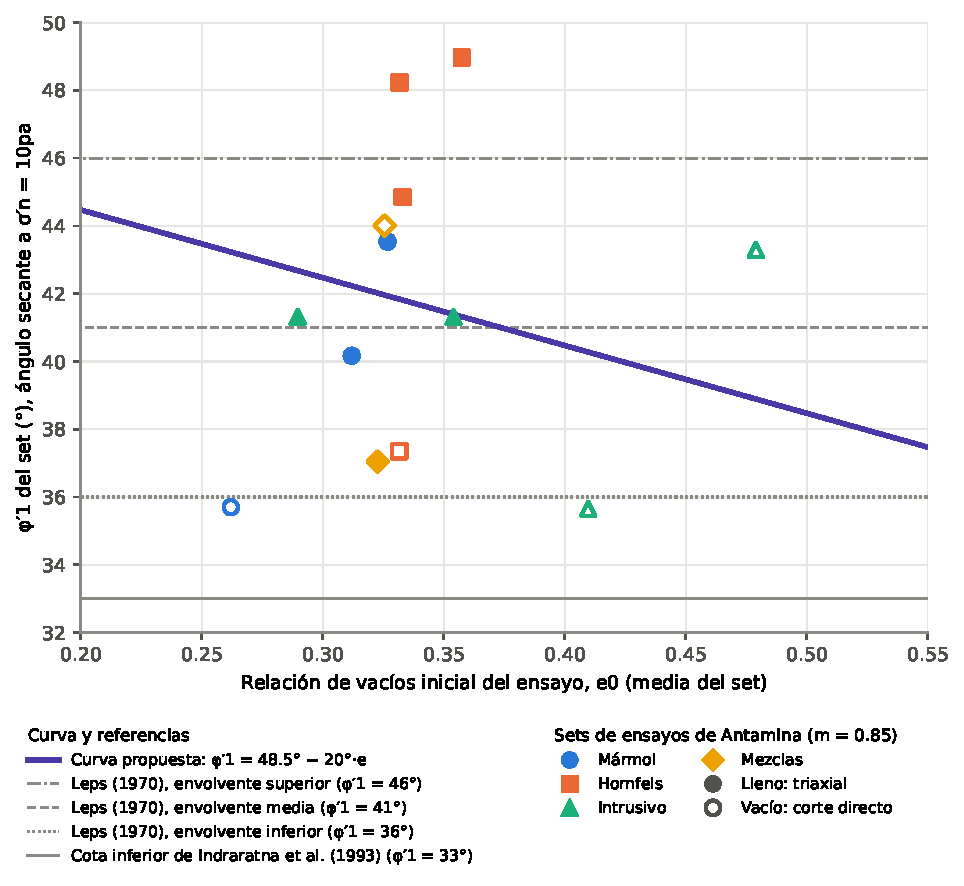
\includegraphics[width=0.85\linewidth]{figs/Fig_phi1_e.pdf}
\caption{$\phi'_1$ de cada set de Antamina (con $m = 0.85$) frente a su $e_0$ media, y la recta de la curva propuesta, $\phi'_1 = 48.5^{\circ} - 20^{\circ}\,e$. En gris, las envolventes de \citet{leps} y la cota inferior de \citet{indraratna1993}, que no dependen de $e$ \citep[p.~2 y Tabla~1]{cylwik}.}\label{fig:phi1e}\end{figure}

\needspace{10\baselineskip}\subsection{Forma: el exponente de la base mundial}
Ajustados solos, los ensayos de Antamina llevan $m$ al límite de Leps 2.0, $m = 1$: el ángulo secante no baja con el esfuerzo. En 6 de los 11 sets con varios esfuerzos el ángulo secante sube con el esfuerzo, y baja en 3. Que el ángulo secante de un enrocado suba con el esfuerzo no es esperable, y probablemente refleja cómo se ensayó: en la mayoría de los triaxiales el máximo desviador llega al final de la carrera, sin pico (sección~\ref{sec:datos}). No se pueden corregir los ensayos con los datos disponibles: todas las probetas de un set tienen la misma $e_0$, y la $e$ después de consolidar solo está en \citet{g2021}. Por eso el exponente se toma de la base mundial de Leps 2.0, con el criterio de que prediga bien los ensayos de mayor esfuerzo, que es donde se usará: $m = 0.85$ (sección~\ref{sec:alto}). La hipótesis $m = 1$ se informa como sensibilidad (Tabla~\ref{tab:hip}).

\needspace{10\baselineskip}\subsection{Relación de vacíos: la de colocación, sin densificación}
La curva se aplica con la $e$ del desmonte al colocarse. El valor base, 0.45, está en el extremo suelto del ROM de Antamina y coincide con la literatura de botaderos altos de volteo (sección~\ref{sec:e}). Las $e_0$ de los ensayos, de 0.26 a 0.48, corresponden a probetas compactadas, no a ROM volteado. La $e$ no se reduce con la profundidad, porque Leps 2.0 se calibró con la $e$ inicial de las probetas: las que se ensayaron a mayor confinamiento también se densificaron al consolidar, y ese efecto ya está en $m$. La densificación con la profundidad se trata como sensibilidad con los perfiles $e(z)$ (sección~\ref{sec:e}), hasta contar con densidad in situ representativa.

\needspace{10\baselineskip}\subsection{Comprobaciones}
La Tabla~\ref{tab:cmp} compara la curva con los ensayos, cada uno con la curva evaluada a su propia $e$. Con los ensayos de Antamina, el sesgo por rango es el costo de no extrapolar su linealidad. Con la base mundial, la diferencia depende de la calidad de la roca: los materiales de calidad buena y moderada son más resistentes que el desmonte de Antamina, y los de calidad baja quedan cerca de la curva. Sobre 4.62~MPa, la curva queda por debajo de la base mundial por la diferencia de material, no por su curvatura, que se verificó con el nivel de cada set.

\begin{table}[!htbp]\centering\small\caption{Ensayos frente a la curva propuesta, cada uno a su $e$: diferencia de $\phi'_s$ (medido menos curva).}\label{tab:cmp}
\begin{tabular}{L{8.6cm}rrr}\toprule Grupo & Ensayos & Mediana (°) & Bajo la curva\\\midrule
Antamina, 0 a 0.5~MPa & 6 & $-$7.4 & 4 \\
Antamina, 0.5 a 2~MPa & 22 & $-$1.3 & 14 \\
Antamina, 2 a 4.62~MPa & 9 & +3.5 & 1 \\
Base mundial, roca de calidad buena, 4.62 a 7.86~MPa & 14 & +5.2 & 0 \\
Base mundial, roca de calidad moderada, 4.62 a 7.86~MPa & 10 & +4.5 & 0 \\
Base mundial, roca de calidad baja, 4.62 a 7.86~MPa & 2 & +0.4 & 1 \\
\bottomrule\end{tabular}\par\vspace{3pt}\footnotesize Calidad de la roca según la clasificación de la base mundial \citep[Tabla~5]{cylwik}.\end{table}

\needspace{10\baselineskip}\section{Resultados}\label{sec:res}
\subsection{Ajuste a los ensayos de Antamina}
Con $m = 0.90$ y todos los ensayos sin ponderar, solo para comparar los escenarios de datos, los tres dan $\phi'_{e=0}$ entre 47.71° y 49.44° (Tabla~\ref{tab:esc}); el escenario de solo gran escala, que excluye las probetas de 6~in y el corte directo, es el más alto. En Leps 2.0 el exponente no puede ser mayor que 1. Si se ajusta $m$ junto con el nivel, los ensayos de Antamina llevan el ajuste a ese límite, $m = 1$: hasta $\sigma'_n \approx 4.6$~MPa la envolvente es prácticamente lineal, sin la curvatura que muestra la base mundial. Por litología, el hornfels y el mármol también llegan al límite, el intrusivo da $m = 0.92$ y el conjunto sin hornfels, $m = 0.96$. La linealidad está influida por el hornfels, cuyo ángulo secante crece con el esfuerzo (de unos 41° a 46° entre 1.7 y 4.6~MPa, antes de la corrección por densidad); sus seis ensayos de gran escala tenían contracción volumétrica en el máximo desviador. Los ensayos de Antamina dan $m \approx 1$, en el límite de Leps 2.0, pero ese valor no se adopta por su representatividad (sección~\ref{sec:alto}). La curva propuesta toma $m = 0.85$ de la base mundial (sección~\ref{sec:alto}).

\begin{table}[!htbp]\centering\small\caption{Ajuste de Leps 2.0 ($\omega = 20^{\circ}$, $m = 0.90$) por escenario de datos, con $\phi'_1$ a $e = 0.45$, y exponente ajustado con el límite de Leps 2.0 ($m \le 1$). Todos los ensayos, sin ponderar por litología.}\label{tab:esc}
\begin{tabular}{lrrrrr}\toprule Escenario & Ensayos & Sets & $\phi'_{e=0}$ (°) & $\phi'_1$ (°) & $m$ ajustado\\\midrule
Todos, con ajuste de escala & 37 & 13 & 47.71 & 38.71 & 1.00 \\
Solo gran escala & 17 & 5 & 49.44 & 40.44 & 1.00 \\
Todos, sin ajuste (base) & 37 & 13 & 48.06 & 39.06 & 1.00 \\
\bottomrule\end{tabular}\end{table}

\needspace{10\baselineskip}\subsection{Rango de esfuerzos con respaldo de datos}\label{sec:rango}
Las figuras y tablas de este memorándum llegan hasta $\sigma'_n = 15$~MPa, pero el respaldo de los datos no es el mismo en todo ese rango. Hay tres zonas:
\begin{itemize}
\item \textbf{Hasta 4.62~MPa}, el máximo de los ensayos de Antamina (triaxial de hornfels con $\sigma'_3 = 2.45$~MPa, convertido con $m = 0.85$). El nivel de la curva se apoya en los ensayos de Antamina y su curvatura, en la base mundial.
\item \textbf{De 4.62 a 7.86~MPa}, el máximo de la base mundial de Leps 2.0, donde solo 34 ensayos, de 29 sets, superan 5~MPa. No hay ensayos de Antamina; la curvatura sigue apoyada en la base mundial y el nivel es el de los ensayos de Antamina a menor esfuerzo.
\item \textbf{Sobre 7.86~MPa}. No hay ensayos en ninguna de las dos fuentes: la curva es una extrapolación de la ley de potencia de Leps 2.0, y la banda se abre en consecuencia.
\end{itemize}
Las figuras marcan estas zonas: gris claro, sin ensayos de Antamina; rayado, fuera de la base mundial. Los valores se extienden hasta 15~MPa porque en un botadero de 700~m el esfuerzo vertical efectivo en la base llega a unos 15.7~MPa con el perfil A (Tabla~\ref{tab:ez}), y una superficie de falla profunda, por ejemplo con fundación débil o compuesta a lo largo de la base, podría movilizar $\sigma'_n$ de ese orden. Fuera de la base mundial, los valores de la curva deben usarse solo como sensibilidad y con la banda completa.

\needspace{10\baselineskip}\subsection{Incertidumbre a alto confinamiento}\label{sec:alto}
La linealidad de Antamina no autoriza a extrapolarla. Su causa no está identificada: puede influir la densificación de las probetas durante la consolidación y los ciclos de carga, pero en la base mundial $m$ casi no se correlaciona con la relación de vacíos ni con el tamaño (ver abajo), de modo que esas propiedades no la explican por sí solas. La decisión de no usar el $m$ de Antamina se basa en no extrapolar fuera de su rango un resultado de 13 sets de un solo sitio, no en una causa demostrada. Por eso el exponente de la curva propuesta se toma de la base mundial de Leps 2.0. En sus 170 sets triaxiales con $\sigma'_3 \ge 0.06$~MPa (la guía 60--600 de \citealp[p.~11]{cylwik}), al menos tres ensayos y $\sigma'_n$ máximo de al menos el doble del mínimo, la pendiente de $\ln\tau$ frente a $\ln\sigma'_n$ (que en Leps 2.0 es $m$) tiene mediana 0.86, P10 de 0.79 y P90 de 0.92. La curvatura se atribuye a la rotura de partículas, que crece con el confinamiento y reduce la dilatancia \citep{marsal1967,indraratna1993}. Para elegir el exponente se buscó el que mejor predice los ensayos mundiales de mayor esfuerzo, que es donde se usará la curva: en cada set con ensayos sobre 4.6~MPa, el nivel se fijó con sus ensayos de menor esfuerzo y se predijeron los de mayor esfuerzo con un $m$ común. El $m$ con residuo mediano nulo es 0.850 (intervalo al 90~\% de 0.834 a 0.862), y la curva propuesta usa $m = 0.85$; la mediana de los sets es 0.86. La banda cubre ese intervalo de $m$. La desviación estándar de las pendientes es 0.064; descontado el error de ajuste de cada set, la dispersión entre materiales es 0.050 (estimador de Paule--Mandel). Las propiedades de los materiales la explican poco: en esos sets, la correlación de Spearman de $m$ con la relación de vacíos, el tamaño máximo, la resistencia de la roca y la rotura es como máximo de 0.12 en valor absoluto, y agregar la relación de vacíos, el tamaño y la clase de roca la reduce poco (0.050 a 0.046). \citet[Tabla~4]{cylwik}, con el coeficiente de Pearson en sus 249 sets, informan correlaciones algo mayores de $m$ con el contenido de grava ($-0.32$) y el $D_{50}$ ($-0.24$), que siguen siendo débiles. Los pares $\sigma'_n$--$\tau$ de la base son los de \citet{cylwik}, que convirtieron los triaxiales con un procedimiento iterativo que considera la curvatura de cada set. Con la información disponible, la incertidumbre de $m$ para Antamina no puede bajar de esa dispersión sin ensayos representativos del campo a alto confinamiento (ítem~4 de la sección~\ref{sec:ensayos}). La base excluyó los ensayos con $\phi'_1 < 31^{\circ}$ \citep[p.~4]{cylwik}, de modo que su distribución de $m$ puede estar sesgada.

Los ensayos de Antamina no se usan para la curvatura. Ajustados con un nivel propio por set, dan $m = 1.00 \pm 0.03$; en una calibración jerárquica con la base mundial, ese resultado pesaría un 69~\% y llevaría $m$ a 0.95. Ese peso refleja solo la dispersión entre ensayos, no su representatividad del botadero.

La incertidumbre de la curva propuesta (sección~\ref{sec:curva}) se representa con una sola banda (Tabla~\ref{tab:hip}, Fig.~\ref{fig:phi}), que reúne dos fuentes:
\begin{itemize}
\item \emph{Curvatura.} $m$ entre 0.834 y 0.862, el intervalo al 90~\% de la prueba con los ensayos mundiales de mayor esfuerzo. Para cada $m$ se reajustó el nivel con los ensayos de Antamina. Las hipótesis no se dibujan una por una: la banda es su envolvente, y sus valores están en la Tabla~\ref{tab:hip}.
\item \emph{Nivel.} El intervalo del nivel al 90~\% (\emph{bootstrap} por sets, estratificado por litología).
\end{itemize}
La hipótesis $m = 1$, que es lo que dan los ensayos de Antamina solos, queda fuera de la banda y se informa como sensibilidad (Tabla~\ref{tab:hip}): daría un ángulo secante constante de 39.0° a $e = 0.45$. Con $m = 0.85$, los ensayos de Antamina quedan en promedio $-$5.4° entre 0 y 0.50~MPa (6 ensayos); $-$1.2° entre 0.5 y 2.00~MPa (22 ensayos); +4.9° entre 2 y 4.62~MPa (9 ensayos) respecto de la curva (medido menos curva): la curva queda sobre ellos a bajo esfuerzo y bajo ellos sobre 2~MPa, el costo de no extrapolar la linealidad de Antamina.

La incertidumbre de la relación de vacíos de colocación no entra en la banda porque se trata explícitamente con las alternativas de $e$ de la sección~\ref{sec:e}; tampoco la de $\omega$ (15--25°), que entra solo en la desviación estándar total de $\phi'_1$ indicada abajo. La banda representa la incertidumbre de la curva media, no la dispersión entre ensayos ni entre litologías: 26 de los 37 ensayos quedan fuera de ella, 12 por encima (sobre todo hornfels e intrusivo) y 14 por debajo. La banda va de 37.4° a 41.7° a 1~MPa, de 34.3° a 38.8° a 2~MPa, de 30.7° a 35.6° a 4.62~MPa y de 28.5° a 33.6° a 8~MPa, y de 26.0° a 31.3° a 15~MPa, ya fuera de la base mundial.

Para análisis probabilísticos, la desviación estándar de $\phi'_{e=0}$ de la curva media es 1.26° (nivel; $m = 0.85$), y la de $\phi'_1$, sumando además $\omega$ entre 15° y 25° y $e$ entre 0.35 y 0.55 (distribuciones uniformes), es 1.75°. Ninguna incluye la variabilidad espacial del botadero.

\begin{table}[!htbp]\centering\small\caption{Ángulo de fricción secante $\phi'_s$ (°) de la curva propuesta a $e = 0.45$ según la hipótesis de curvatura, con el nivel ajustado a los ensayos, y límites de la banda de incertidumbre.}\label{tab:hip}
\setlength{\tabcolsep}{4.5pt}\begin{tabular}{lrrrrrrrr}\toprule Hipótesis & $m$ & $\phi'_{e=0}$ (°) & 1~MPa & 2~MPa & 3~MPa & 4.62~MPa & 8~MPa$^{w}$ & 15~MPa$^{w}$\\\midrule
$m$ alto (IC 90~\%) & 0.862 & 48.43 & 39.5 & 36.8 & 35.3 & 33.7 & 31.7 & 29.5 \\
Curva propuesta & 0.850 & 48.47 & 39.5 & 36.6 & 35.0 & 33.3 & 31.1 & 28.8 \\
$m$ bajo (IC 90~\%) & 0.834 & 48.53 & 39.6 & 36.4 & 34.6 & 32.7 & 30.3 & 27.8 \\
Antamina sola$^{s}$ & 1.000 & 48.03 & 39.0 & 39.0 & 39.0 & 39.0 & 39.0 & 39.0 \\
\midrule Banda, límite inferior & & & 37.4 & 34.3 & 32.6 & 30.7 & 28.5 & 26.0 \\
Banda, límite superior & & & 41.7 & 38.8 & 37.2 & 35.6 & 33.6 & 31.3 \\
\bottomrule\end{tabular}\par\vspace{3pt}\footnotesize $^{s}$Sensibilidad: el exponente de los ensayos de Antamina solos; no entra en la banda. $^{w}$Sobre el máximo de la base mundial de Leps 2.0 (7.86~MPa): extrapolación fuera de toda la data (sección~\ref{sec:rango}).\end{table}

\begin{figure}[!htbp]\centering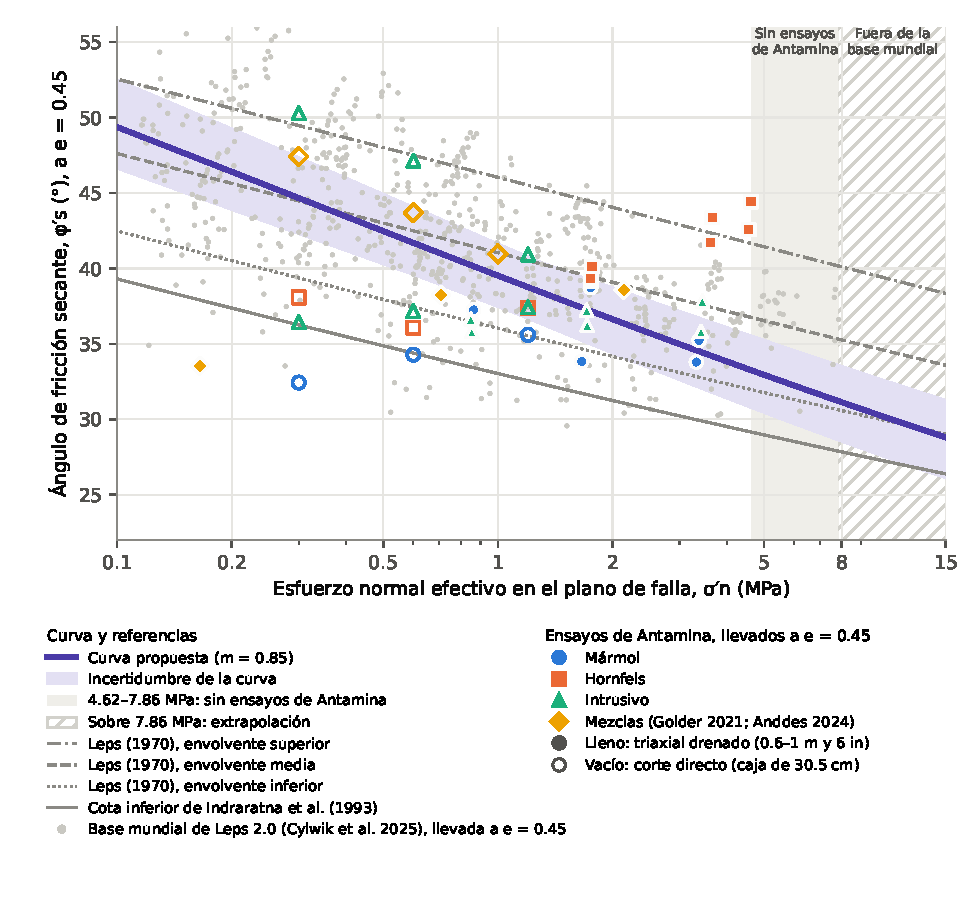
\includegraphics[width=\linewidth]{figs/Fig1_phi_sigma.pdf}
\caption{Curva propuesta ($m = 0.85$) y su banda de incertidumbre, con los ensayos del ajuste llevados a $e = 0.45$ (Ec.~27 de Leps 2.0), y en gris claro los ensayos de la base mundial de Leps 2.0 \citep{cylwik}, llevados a la misma $e$. Color y forma por litología; marcador lleno: triaxial drenado (probetas de 0.6--1~m y de 6~in); vacío: corte directo de gran escala (caja de 30.5~cm). En gris, como referencia, las envolventes superior, media e inferior de \citet{leps} ($\phi'_1$ = 46°, 41° y 36°) y la cota inferior de \citet{indraratna1993} ($\phi'_1 = 33^{\circ}$), todas en la forma de la Ec.~9 de Leps 2.0 ($m = 0.9$; \citealp[p.~2 y Tabla~1]{cylwik}), que no depende de $e$. Zona gris: entre el máximo $\sigma'_n$ de los ensayos de Antamina (4.62~MPa) y el de la base mundial (7.86~MPa); rayado: fuera de la base mundial (sección~\ref{sec:rango}).}\label{fig:phi}\end{figure}

\needspace{10\baselineskip}\subsection{Contraste con los ensayos no usados en el ajuste}\label{sec:contraste}
La Fig.~\ref{fig:contraste} compara la curva con los triaxiales no drenados (CU) de desmonte ROM, que no entran en el ajuste (los de la fase A de \citealp{g2010} y los de \citealp{anddes2024}), llevados a $e = 0.45$ con la misma corrección por densidad. Se convirtieron a $\sigma'_n$--$\tau$ con los esfuerzos efectivos en la falla y la misma conversión de Leps 2.0 que los drenados. Respecto de la curva propuesta, la diferencia media de $\phi'_s$ es:
\begin{itemize}
\item triaxiales CU de 6~in de \citet{anddes2024}, a máxima oblicuidad (15 ensayos): +2.5°;
\item triaxiales CU de 2.8 y 4~in de la fase A de \citet{g2010}, al máximo desviador, único criterio que informa el laboratorio (21 ensayos): $-$7.4°.
\end{itemize}
Los CU quedan a ambos lados de la curva y no son comparables con el ajuste. Su resistencia depende de la presión de poros y del criterio de falla: el laboratorio de \citet{anddes2024} toma la falla al 15~\% de deformación, y en 12 de sus 15 probetas el desviador seguía creciendo. Además, los de \citet{g2010} son probetas pequeñas, con la gradación cortada a 9.5--15.9~mm, y parte se remoldeó a la densidad mínima ($e$ de 0.49 a 0.54) y el resto a una compacidad mayor ($e$ de 0.27 a 0.45; \citealp[p.~4]{g2010}). La $e$ de los CU de \citet{anddes2024} se calculó igual que la de sus cortes directos, con el $G_s$ de \citet{g2010}.

\begin{figure}[!htbp]\centering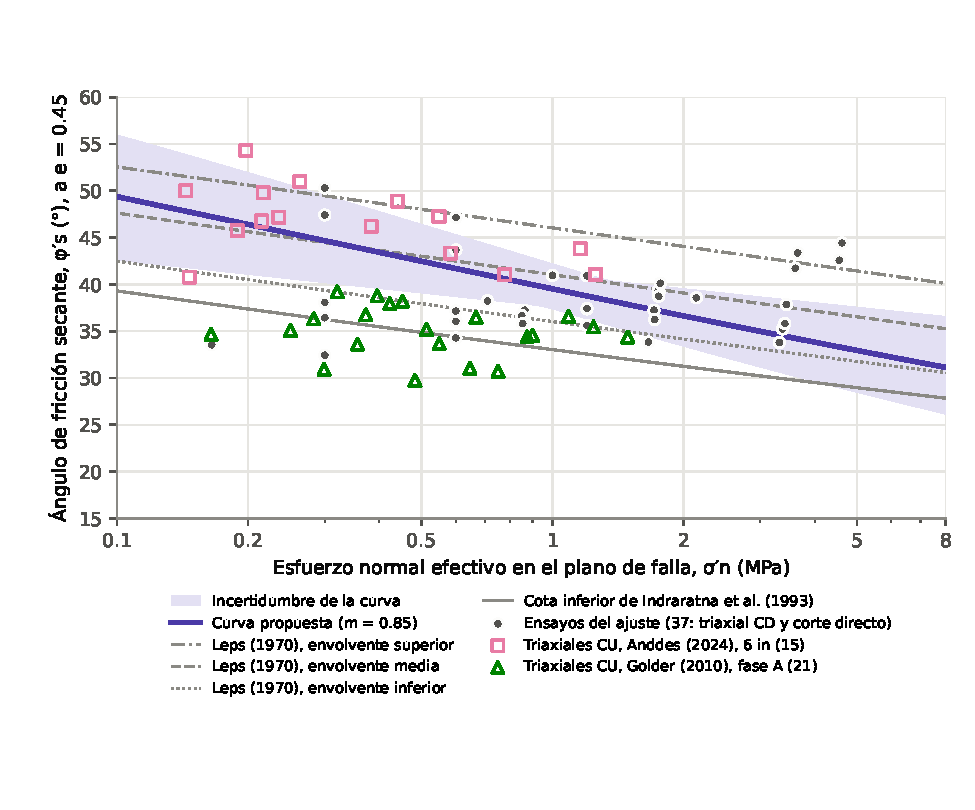
\includegraphics[width=\linewidth]{figs/Fig4_contraste.pdf}
\caption{Contraste de la curva propuesta con los triaxiales CU de desmonte ROM no usados en el ajuste, llevados a $e = 0.45$: \citet{anddes2024} y fase A de \citet{g2010}. Puntos grises: ensayos del ajuste (triaxiales drenados y cortes directos).}\label{fig:contraste}\end{figure}

\needspace{10\baselineskip}\subsection{Rotura de partículas}\label{sec:rotura}
16 de los triaxiales drenados del ajuste tienen el índice de rotura de \citet{marsal1967}, $B_g$, informado o recalculado de las granulometrías antes y después del ensayo (Fig.~\ref{fig:bg}). En \citet{g2012} se usa el valor recalculado, porque la Tabla~5 del informe da la suma de las diferencias absolutas, que es el doble de $B_g$. $B_g$ va de 8 a 39~\% con $\sigma'_3$ de 0.49 a 2.45~MPa y crece con el confinamiento ($B_g \approx 7.5 + 11\,\sigma'_3$, con $\sigma'_3$ en MPa; $r = 0.79$). Es mayor en el hornfels (15--39~\%) y el mármol (13--30~\%) que en el intrusivo (8--18~\%).

La rotura ya es importante a 1--2.5~MPa: con $\sigma'_3$ de 0.98 a 2.45~MPa, $B_g$ va de 8.5 a 39~\%, y en el hornfels y el mármol de gran escala, de 20 a 39~\%: una parte apreciable de las partículas se fragmenta durante el ensayo. En la literatura, la rotura es el mecanismo al que se atribuye la curvatura de la envolvente a alto confinamiento \citep{marsal1967,indraratna1993}. En la base de Leps 2.0, sin embargo, $B_g$ apenas se correlaciona con $m$ (sección~\ref{sec:alto}), y en los ensayos de Antamina una rotura de hasta 39~\% no curvó la envolvente hasta 4.62~MPa. La rotura no justifica por sí sola la curvatura sobre ese esfuerzo; la justificación es la base mundial. La rotura también aumenta con el tamaño de partícula, lo que se trata en la sección~\ref{sec:tamano}. Con un solo valor de $B_g$ por ensayo, y sin ensayos sobre 2.45~MPa, los datos no permiten cuantificar la curvatura a partir de la rotura.

\begin{figure}[!htbp]\centering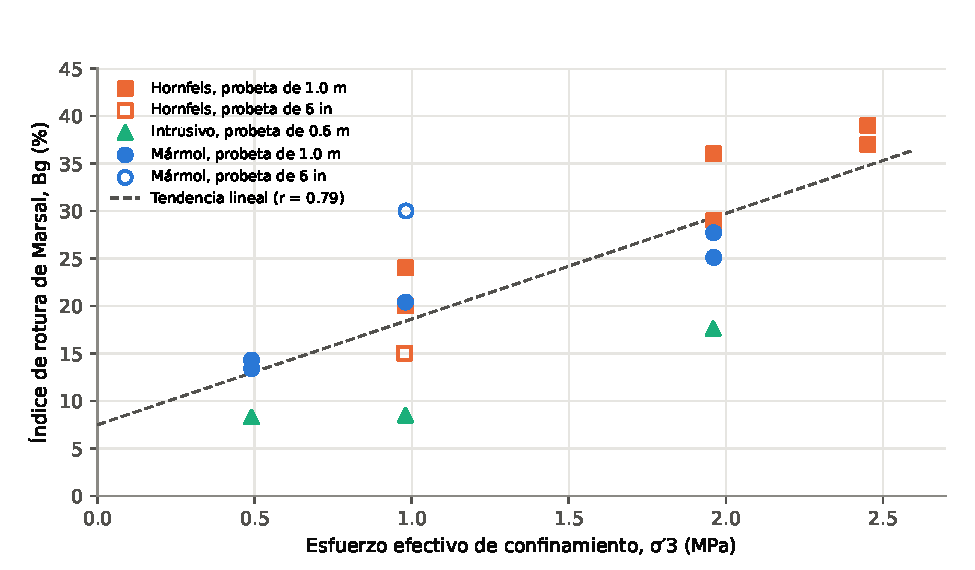
\includegraphics[width=0.9\linewidth]{figs/Fig5_bg.pdf}
\caption{Índice de rotura de \citet{marsal1967} en los triaxiales drenados del ajuste, según el esfuerzo efectivo de confinamiento. Símbolos llenos: probetas de 0.6 y 1~m; vacíos: probetas de 6~in.}\label{fig:bg}\end{figure}

\needspace{10\baselineskip}\section{Curva propuesta}\label{sec:curva}
Stantec propone una curva de Leps 2.0 para el desmonte ROM, con el nivel anclado a los ensayos de Antamina y la curvatura de la base mundial ($m = 0.85$). La curva trata el desmonte como un solo material, como el diseño del DDE \citep[Tabla~3-1]{stantec2026iff}: se ajustó con los 37 ensayos de Antamina con igual peso: los de mármol, hornfels e intrusivo y las dos mezclas (el compuesto de \citealp{g2021}, triaxial de 6~in, y la pila 01 de mármol y hornfels de \citealp{anddes2024}, corte directo), que representan desmonte mezclado:
\begin{equation}
\tau = \tan\!\left(48.47^{\circ} - 20^{\circ}\,e\right)\,(10p_a)^{0.150}\,\sigma_n'^{\,0.850},\qquad \phi'_1(e = 0.45) = 39.47^{\circ}
\end{equation}
Como control, el DDE incluye en sus bases de diseño la producción de desmonte por litología desde 2021: intrusivo y exoskarn, 44~\%, y hornfels y mármol, 56~\% \citep[Tabla~3-1]{stantec2026iff}. Ponderar los ensayos de las tres litologías con esas fracciones (con el 56~\% repartido por igual entre hornfels y mármol, que el DDE no separa, y el 44~\% asignado al intrusivo, porque no hay ensayos de exoskarn) da $\phi'_{e=0} = 48.42^{\circ}$, prácticamente la misma curva. El mármol es la litología ensayada más débil (sección~\ref{sec:vacios}). Comparada con la cota inferior de \citet{hc2017} para construcción descendente de botaderos de peligro muy alto o alto ($\tau = 1.446\,\sigma^{0.898}$ en kPa, Tabla~5.9, propuesta para enrocado de calidad alta y moderada), la curva propuesta queda +3.97° a 1~MPa, +2.40° a 3~MPa y +1.10° a 8~MPa. Con $e = 0.45$, la curva propuesta queda sobre esa cota genérica, y 29 de los 37 ensayos llevados a esa $e$ quedan sobre ella; la diferencia depende principalmente de la $e$ de colocación (sección~\ref{sec:e}).

\citet[Fig.~13, p.~49]{indraratna1993} propusieron un límite inferior para la resistencia de enrocados, 3° bajo el límite inferior que \citet{leps} había dado para enrocado de baja densidad, trazado entre unos 7~kPa y 3.5~MPa. \citet[p.~13]{cylwik} lo compararon con los ensayos de enrocados de calidad baja de su base ($e > 0.45$), normalizados a $e = 0.6$, encontraron que captura el borde inferior de esos datos y lo reproducen con su Ec.~9, $m = 0.9$ y $\phi'_1 = 33^{\circ}$. Esos ensayos llegan a $\sigma'_n \approx 0.75$~MPa \citep[Fig.~19]{cylwik}, de modo que sobre ese esfuerzo la forma con $m = 0.9$ es una extrapolación. No es un ángulo mínimo constante: su ángulo secante también baja con el esfuerzo. En esa forma no depende de $e$ \citep[Tabla~1]{cylwik} y queda 3° bajo la envolvente inferior de \citet{leps}; da 33.0° a 1~MPa, 29.2° a 4.62~MPa y 27.8° a 8~MPa (Figs.~\ref{fig:phi} y~\ref{fig:tau}). La curva propuesta queda +6.5° sobre esa forma a 1~MPa, +4.1° a 4.62~MPa, +3.3° a 8~MPa y +2.41° a 15~MPa, y sobre ella en todo el rango hasta 15~MPa. Sobre 4.62~MPa las dos son extrapolaciones: la curva propuesta, de los ensayos de Antamina (sección~\ref{sec:rango}), y la cota, de ensayos que llegan a unos 0.75~MPa. La cota no se usa para acotar la banda, porque 3 de los 37 ensayos de Antamina quedan por debajo de ella, 3 con $\sigma'_n \le 0.6$~MPa; los más alejados son la mezcla triaxial de 6~in de \citet{g2021} a 0.16~MPa (4.4° por debajo) y los cortes directos de la ruma de mármol ROM (hasta 3.8° por debajo). \citet{cylwik} advierten, además, que su base no tiene rocas con resistencia a la compresión menor que 25~MPa y que materiales más débiles pueden quedar bajo sus predicciones.

\textbf{A grandes esfuerzos.} Sobre 4.62~MPa la curva no tiene ensayos de Antamina, así que conviene contrastarla con los ensayos más altos disponibles, cada uno con la curva evaluada a su propia $e$. Entre 4.62 y 7.86~MPa, 25 de los 26 ensayos de la base mundial quedan sobre la curva, con una mediana de +5.1° en $\phi'_s$, y de los 8 ensayos de Antamina con $\sigma'_n$ sobre 3~MPa, 7 quedan sobre ella (mediana +5.4°): la curva queda del lado conservador a grandes esfuerzos. A 10~MPa da 30.3°, sobre la cota de \citet{indraratna1993} (27.3°) y la de \citet{hc2017} (29.5°), y bajo los 33° que el DDE usó como sensibilidad entre 5 y 10~MPa de esfuerzo vertical efectivo, con 30° por encima \citep[§3.5.3.6, Tabla~3-24, nota~4]{stantec2026iff}; en la base de una dovela, $\sigma'_n \le \sigma'_v$.

El exponente $m = 0.85$ es el que predice sin sesgo los ensayos mundiales de mayor esfuerzo (sección~\ref{sec:alto}), algo menor que el valor estándar del modelo simplificado (0.9). Las hipótesis de curvatura, incluida $m = 1$, están en la Tabla~\ref{tab:hip}.

\textbf{Posición frente a \citet{leps}.} Las envolventes de \citet{leps}, en la forma de Leps 2.0 ($\phi'_1$ = 36°, 41° y 46° con $m = 0.9$; \citealp[p.~2]{cylwik}), no dependen de $e$: la densidad está en la clase (baja densidad, promedio, alta densidad). Por eso la posición de la curva propuesta frente a ellas depende de la $e$ con que se la evalúe. Con $e = 0.45$ constante, la curva cruza la envolvente media a 0.34~MPa, queda entre la media y la inferior sobre ese esfuerzo y alcanza la inferior a unos 12.4~MPa, porque su $m$ es menor que 0.9. Con la $e$ del perfil A, que baja con la profundidad (sección~\ref{sec:e}), la curva sigue a la envolvente media: en una escala en que 0 es la envolvente inferior y 1 la media, su posición es 1.09, 0.97, 0.89, 0.85 a 1, 4, 10 y 15~MPa. Para comparar con \citet{leps}, la $e$ de colocación pesa tanto como la curva misma.

\subsection*{Comportamiento a bajo confinamiento}
Las curvas se entregan sin tope. Con $m < 1$, el ángulo secante de Leps 2.0 crece al bajar $\sigma'_n$ y supera el ángulo de reposo de las caras de volteo de Antamina (típicamente 37° en caras de volteo; \citealp[§16.5]{hc2017}) bajo $\sigma'_n$ = 1.83~MPa con $e = 0.45$. \citet{cylwik} indican que bajo 0.1~MPa el criterio tiende a subestimar la resistencia medida. Para el desmonte suelto de la cara, en cambio, la resistencia movilizable está cerca del ángulo de reposo. Con $\sigma'_n$ menor que 0.5~MPa hay 6 ensayos: la mezcla triaxial de \citet{g2021} (6~in, $\sigma'_3 = 0.10$~MPa, máximo desviador con 4.0~\% de deformación axial) y los cortes directos a 0.3~MPa. Llevados a $e = 0.45$, sus ángulos van de 32.4° a 50.3°, frente a unos 45° de la curva: 4 quedan bajo la curva y 2 sobre ella. A bajo confinamiento los ensayos son pocos y muy dispersos, y no respaldan la curva de forma consistente.

Por eso, la curva sin tope se entrega con una condición de aplicación: los mecanismos de cara y de banco, con $\sigma'_n$ menor que el cruce con 37° (1.8~MPa), se verifican además con $\phi' = 37^{\circ}$. \citet[§8.4.1.1]{hc2017} indican que el peligro de inestabilidad superficial de las caras a ángulo de reposo se maneja normalmente con procedimientos operacionales, y que analizarlo no suele aportar, porque su factor de seguridad es 1 por definición. Por eso la verificación con 37° tiene sentido en caras y bancos más tendidos que el ángulo de reposo.

\needspace{10\baselineskip}\section{Valores para los modelos de equilibrio límite}\label{sec:valores}
La Tabla~\ref{tab:slide} da los pares $\sigma'_n$--$\tau$ de la curva propuesta a $e = 0.45$ y de los límites de su incertidumbre, y la Tabla~\ref{tab:slide_e}, los de la curva propuesta para cada supuesto de $e$. Ambas incluyen el origen y puntos desde 10~kPa, para definir la curva cerca del origen. Las curvas con $e$ constante también pueden cargarse como función de potencia (\emph{Power Curve} de Slide2, $\tau = a(\sigma'_n + d)^b + c$), con los parámetros de la Tabla~\ref{tab:power}. Los perfiles $e(z)$ no son una función de potencia y se cargan como pares. La Fig.~\ref{fig:tau} compara la curva propuesta con las envolventes de \citet{leps} y la cota inferior de \citet{indraratna1993}.

\begin{table}[!htbp]\centering\small\caption{Pares $\sigma'_n$--$\tau$ a $e = 0.45$: curva propuesta y límites de su incertidumbre.}\label{tab:slide}
\begin{tabular}{rrrrr}\toprule $\sigma'_n$ & $\tau$ curva propuesta & $\tau$ límite inferior$^{b}$ & $\tau$ límite superior$^{b}$ & $\phi'_s$ curva propuesta\\
(kPa) & (kPa) & (kPa) & (kPa) & (°)\\\midrule
0 & 0.0 & 0.0 & 0.0 & -- \\
10 & 16.5 & 14.5 & 19.1 & 58.7 \\
20 & 29.7 & 26.4 & 34.1 & 56.0 \\
30 & 41.9 & 37.4 & 47.8 & 54.4 \\
50 & 64.7 & 58.1 & 73.2 & 52.3 \\
100 & 116.5 & 105.7 & 130.6 & 49.4 \\
200 & 210.1 & 192.1 & 232.7 & 46.4 \\
500 & 457.7 & 423.1 & 499.7 & 42.5 \\
1000 & 825.1 & 764.8 & 890.8 & 39.5 \\
1500 & 1164.6 & 1074.4 & 1254.1 & 37.8 \\
2000 & 1487.2 & 1365.8 & 1607.1 & 36.6 \\
3000 & 2099.1 & 1915.3 & 2279.4 & 35.0 \\
4000 & 2680.7 & 2434.6 & 2920.9 & 33.8 \\
5000$^{a}$ & 3240.5 & 2932.6 & 3540.5 & 32.9 \\
6000$^{a}$ & 3783.7 & 3414.2 & 4143.0 & 32.2 \\
8000$^{a,w}$ & 4831.9 & 4340.0 & 5309.0 & 31.1 \\
10000$^{a,w}$ & 5841.0 & 5227.7 & 6435.0 & 30.3 \\
12000$^{a,w}$ & 6820.2 & 6086.3 & 7530.1 & 29.6 \\
15000$^{a,w}$ & 8244.6 & 7331.2 & 9127.2 & 28.8 \\
\bottomrule\end{tabular}\par\vspace{3pt}\footnotesize $^{a}$Sobre el máximo $\sigma'_n$ de los ensayos de Antamina (4.62~MPa). $^{w}$Sobre el máximo de la base mundial de Leps 2.0 (7.86~MPa): extrapolación fuera de toda la data (sección~\ref{sec:rango}). $^{b}$Límites de incertidumbre para sensibilidad; no son valores de diseño. Bajo 0.5~MPa hay pocos ensayos y muy dispersos.\end{table}

\begin{table}[!htbp]\centering\small\caption{Pares $\sigma'_n$--$\tau$ (kPa) de la curva propuesta según la relación de vacíos y de la recta de 37° para verificar caras y bancos.}\label{tab:slide_e}
\setlength{\tabcolsep}{4pt}\begin{tabular}{rrrrrrr}\toprule $\sigma'_n$ & $e = 0.45$ & $e = 0.55$ & $e = 0.65$ & Perfil A & Perfil V & $\phi' = 37^{\circ}$\\
(kPa) & (base) & & & & & \\\midrule
0 & 0.0 & 0.0 & 0.0 & 0.0 & 0.0 & 0.0 \\
10 & 16.5 & 15.3 & 14.2 & 16.5 & 16.5 & 7.5 \\
20 & 29.7 & 27.6 & 25.7 & 29.7 & 29.7 & 15.1 \\
30 & 41.9 & 39.0 & 36.2 & 41.9 & 41.9 & 22.6 \\
50 & 64.7 & 60.2 & 55.9 & 64.7 & 64.8 & 37.7 \\
100 & 116.5 & 108.5 & 100.8 & 118.4 & 117.0 & 75.4 \\
200 & 210.1 & 195.5 & 181.8 & 216.9 & 211.9 & 150.7 \\
500 & 457.7 & 426.1 & 396.1 & 482.6 & 467.6 & 376.8 \\
1000 & 825.1 & 768.0 & 713.9 & 883.8 & 858.9 & 753.6 \\
1500 & 1164.6 & 1084.0 & 1007.7 & 1265.3 & 1231.8 & 1130.3 \\
2000 & 1487.2 & 1384.3 & 1286.8 & 1632.1 & 1596.9 & 1507.1 \\
3000 & 2099.1 & 1953.9 & 1816.3 & 2336.6 & 2318.7 & 2260.7 \\
4000 & 2680.7 & 2495.2 & 2319.5 & 3013.9 & 3038.6 & 3014.2 \\
5000$^{a}$ & 3240.5 & 3016.4 & 2803.9 & 3671.8 & 3748.1 & 3767.8 \\
6000$^{a}$ & 3783.7 & 3522.0 & 3273.9 & 4314.6 & 4455.7 & 4521.3 \\
8000$^{a,w}$ & 4831.9 & 4497.6 & 4180.8 & 5565.2 & 5834.4 & 6028.4 \\
10000$^{a,w}$ & 5841.0 & 5437.0 & 5054.0 & 6780.0 & 7212.7 & 7535.5 \\
12000$^{a,w}$ & 6820.2 & 6348.4 & 5901.2 & 7966.8 & 8540.9 & 9042.6 \\
15000$^{a,w}$ & 8244.6 & 7674.3 & 7133.7 & 9705.7 & -- & 11303.3 \\
\bottomrule\end{tabular}\par\vspace{3pt}\footnotesize $^{a}$Sobre el máximo $\sigma'_n$ de los ensayos de Antamina (4.62~MPa). $^{w}$Sobre el máximo de la base mundial (7.86~MPa): extrapolación fuera de toda la data. Perfil V: sin valores sobre $\sigma'_v \approx 13.9$~MPa, donde termina la curva de Valenzuela et al.\ (600~m de altura).\end{table}

\begin{table}[!htbp]\centering\small\caption{Parámetros de \emph{Power Curve} de Slide2 ($\tau = a(\sigma'_n + d)^b + c$, con $\sigma'_n$ y $\tau$ en kPa), equivalentes a Leps 2.0 con $e$ constante: $a = \tan\phi'_1 \cdot 1013^{1-m}$, $b = m$.}\label{tab:power}
\begin{tabular}{lrrrrrrr}\toprule Curva & $\phi'_{e=0}$ (°) & $e$ & $\phi'_1$ (°) & $a$ & $b$ & $c$ (kPa) & $d$ (kPa)\\\midrule
Curva propuesta & 48.47 & 0.45 & 39.47 & 2.3254 & 0.8500 & 0 & 0 \\
Curva propuesta & 48.47 & 0.55 & 37.47 & 2.1645 & 0.8500 & 0 & 0 \\
Curva propuesta & 48.47 & 0.65 & 35.47 & 2.0120 & 0.8500 & 0 & 0 \\
\bottomrule\end{tabular}\end{table}

\begin{figure}[!htbp]\centering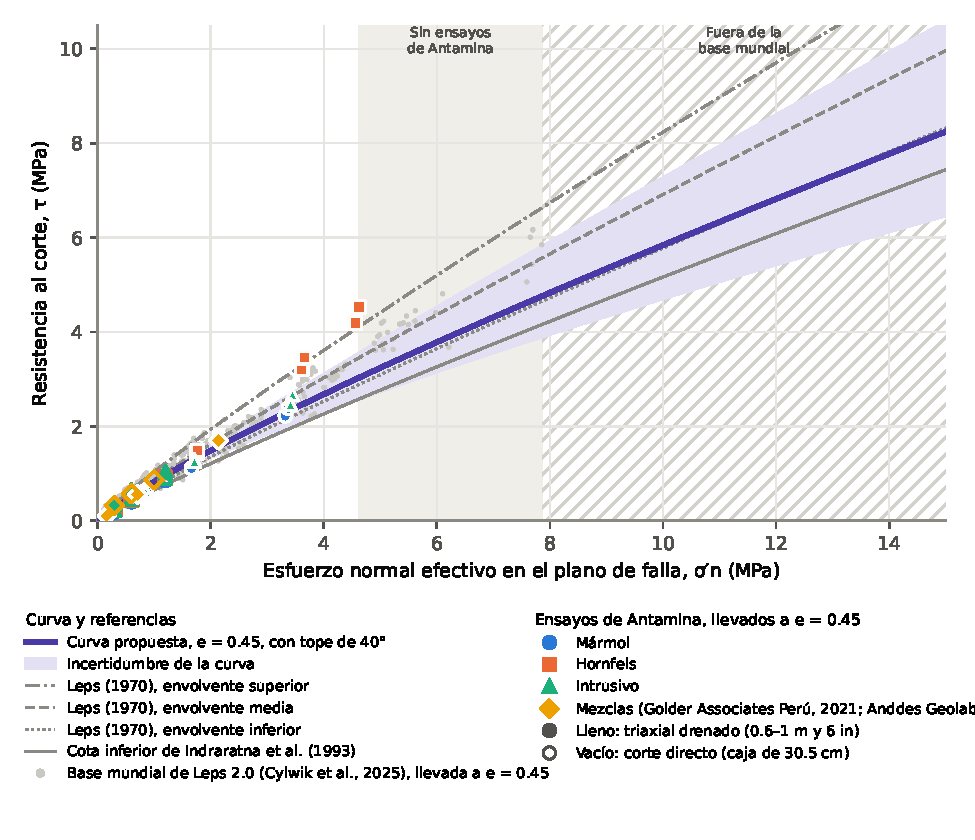
\includegraphics[width=\linewidth]{figs/Fig2_tau_sigma.pdf}
\caption{Curva propuesta y su banda de incertidumbre en $\tau$--$\sigma'_n$, con los ensayos drenados llevados a $e = 0.45$ (incluidas las dos mezclas) y, en gris claro, la base mundial de Leps 2.0 llevada a la misma $e$. En gris, como referencia: las envolventes superior, media e inferior de \citet{leps} y la cota inferior de \citet{indraratna1993}, en la forma de la Ec.~9 de Leps 2.0 ($m = 0.9$; \citealp[p.~2 y Tabla~1]{cylwik}).}\label{fig:tau}\end{figure}

\needspace{10\baselineskip}\section{Relación de vacíos de colocación}\label{sec:e}
La $e$ de colocación es el supuesto que más mueve la curva: cada 0.05 de $e$ cambia $\phi'_1$ en 1°. La $e$ depende de cómo se coloca el material, y en Antamina hay tres materiales de desmonte con colocación distinta:
\begin{itemize}
\item \textbf{Desmonte ROM}, descargado de camiones y volteado sin compactar, con tamaño máximo de partícula del orden de 1~m \citep[Tabla~3-1]{stantec2026iff}: es el más suelto. Es el material de esta curva.
\item \textbf{Desmonte chancado}, más fino y mejor gradado, colocado con fajas sin compactar: es más denso que el ROM.
\item \textbf{Enrocado 3B} de la presa de relaves, colocado en capas y compactado con rodillo: es el más denso. Parte de los ensayos del ajuste son de este material (sección~\ref{sec:datos}).
\end{itemize}
La $e$ in situ del ROM no se ha medido directamente, pero los pesos unitarios que miden y adoptan los estudios de Antamina permiten calcularla (Tabla~\ref{tab:ebase}). Para el ROM dan $e$ de 0.25 a 0.45, con el valor más bajo medido en la superficie de un botadero; la literatura da 0.25 a 0.9, con 0.45 a 0.49 en botaderos altos de volteo. El valor base, 0.45, está en el extremo suelto del rango de Antamina y en el de la literatura: es representativo del ROM volteado y queda del lado conservador. El chancado y el enrocado dan $e$ de 0.25 a 0.28, claramente más densos; por eso los ensayos de enrocado compactado ($e_0$ de 0.30 a 0.34) se llevan a la $e$ del ROM con la regla de densidad de Leps 2.0 antes de ajustar la curva. El valor base está dentro del rango de los ensayos ($e_0$ = 0.262--0.479), así que esa corrección no extrapola la regla. Con 0.65, más suelto que toda la evidencia y que la categoría «suelta» de Leps 2.0, la curva representaría el material más suelto de la cara de volteo; 0.55 y 0.65 se entregan como sensibilidad conservadora.

\begin{table}[!htbp]\centering\small\caption{Relación de vacíos de colocación del desmonte de Antamina según el material, calculada con los pesos unitarios de los estudios de Antamina, y valores de la literatura.}\label{tab:ebase}
\begin{tabular}{L{2.0cm}L{8.4cm}r>{\raggedleft\arraybackslash}p{2.1cm}}\toprule Material & Fuente & $\gamma$ (kN/m³) & $e$\\\midrule
ROM & Pesos unitarios totales medidos in situ en Antamina, con dispersión de 19 a 24~kN/m³; valor adoptado \citep[pp.~12--14, Fig.~4 y Tabla~3]{stantec2025sda} & 20.0 & 0.39\\
ROM & Diseño geotécnico del DDE \citep[Tabla~9-3]{stantec2026dde} & 19.6 & 0.42\\
ROM & Densidad del desmonte para el tonelaje del plan, 1.95~t/m³ \citep[Tabla~4-1]{stantec2026dde} & -- & 0.41--0.45$^{a}$\\
ROM & Densidad por reemplazo de agua en la superficie del Botadero Tucush, junto al sondaje BH19-BT-01; probablemente compactada por el tránsito \citep[Anexo~C, Tabla~3]{wsp2023tsf} & -- & 0.25$^{b}$\\
ROM & Peso unitario total promedio de \citet{g2010}, citado en \citet[p.~59]{stantec2026dde} & 20.75 & 0.34\\
Chancado & \citet{g2010}, citado en \citet[p.~59]{stantec2026dde} & 21.66 & 0.28\\
Chancado & Valor adoptado \citep[Tabla~3]{stantec2025sda} & 22.0 & 0.26\\
Enrocado 3B & Diseño geotécnico del DDE \citep[Tabla~9-3]{stantec2026dde} y \citet[Tabla~3]{stantec2025sda} & 22.0 & 0.26\\
\midrule
Literatura & \citet[Fig.~10]{valenzuela2008}, envolvente propuesta, en superficie ($\gamma_d \approx 1.84$~t/m³) & -- & 0.49\\
Literatura & \citet[§5.5.1.6]{hc2017}: botaderos (Dawson et al. 1998), Andina (Linero et al. 2006) y medidos en terreno (Golder Associates 1987) & -- & 0.4--0.9; 0.46; 0.25--0.3\\
Literatura & Leps 2.0 \citep[Tabla~6]{cylwik}: densa, media y suelta & -- & 0.30; 0.45; 0.60\\
\bottomrule\end{tabular}\par\vspace{3pt}\footnotesize $e = G_s\,\gamma_w\,(1 + w)/\gamma - 1$, con $G_s$ = 2.75, $\gamma_w$ = 9.81~kN/m³ y la humedad informada en \citet[Tabla~3]{stantec2025sda} (2.9~\% en el ROM y 2.8~\% en el chancado). $^{a}$Densidad seca o húmeda: el informe no lo indica. $^{b}$Densidad seca medida de 2.200~t/m³.\end{table}

La $e$ de la curva es constante y no baja con el esfuerzo, aunque el desmonte se comprime con la profundidad. Hay dos razones. Primero, Leps 2.0 se calibró con la $e$ inicial de cada probeta, antes de consolidar: en su base, las probetas ensayadas a mayor confinamiento también se densificaron al consolidar, y ese efecto ya está dentro de la curvatura $m$. Bajar además la $e$ con la profundidad contaría dos veces la densificación. Segundo, la compresibilidad del ROM suelto en el botadero no se ha medido en Antamina. La densificación con la profundidad se evalúa aparte, como sensibilidad, con los perfiles $e(z)$ de esta sección.
 La $e$ de un botadero alto, además, no es constante: el desmonte se comprime y rompe con la carga, y \citet[Fig.~10]{valenzuela2008} propusieron, a partir de triaxiales y edómetros de gran escala, una envolvente de densidad seca que crece de unos 1.84 a 2.37~t/m³ entre la superficie y 600~m de altura ($e$ de 0.49 a 0.16 con $G_s = 2.75$; la figura está reproducida en \citealp[Fig.~5.6]{hc2017}). La evolución que adoptaron para el diseño de un botadero alto es escalonada y más conservadora, de 1.86 a 2.25~t/m³.

Por eso se entregan, para la curva propuesta (Fig.~\ref{fig:e}, Tablas~\ref{tab:ez}, \ref{tab:etau} y~\ref{tab:slide_e}):
\begin{itemize}
\item \textbf{$e$ constante de 0.45, 0.55 y 0.65}, para asignar por sectores o como sensibilidad.
\item \textbf{Perfiles $e(z)$ con densificación}, partiendo de $e = 0.45$ en superficie. El perfil A usa la compresibilidad de la rama de carga del edómetro de mármol más suelto de Antamina (probeta de 0.24~m, $e_0 = 0.455$ con $G_s = 2.70$ supuesto; \citealp{w2022}): $C_c$ = 0.075 entre 0.2 y 0.8~MPa y 0.115 entre 1.2 y 4.8~MPa, extrapolado fuera de ese rango. El perfil V usa la forma de la envolvente propuesta por \citet{valenzuela2008}, leída de la figura y desplazada para partir de $e = 0.45$; no es su curva de diseño, que es escalonada. Se usa la envolvente porque resume la tendencia de los ensayos de gran escala y es continua. Con la curva de diseño, desplazada de la misma manera, la $e$ a 600~m sería 0.19 en vez de 0.12: el perfil V es, por eso, la más favorable de las alternativas de densificación, y se entrega como sensibilidad. A cada $\sigma'_n$ se le asigna la $e$ de la profundidad donde $\sigma'_v = \sigma'_n$; como en la base de una dovela $\sigma'_n \le \sigma'_v$, eso usa una $e$ algo más suelta que la real.
\end{itemize}
El perfil A llega a $e \approx 0.22$ a 700~m y el V a $e \approx 0.12$ a 600~m. A 8~MPa dan 34.8° (A) y 36.1° (V), frente a 31.1° con $e = 0.45$ constante: con densificación, la envolvente se acerca a la linealidad de los ensayos de Antamina, cuyas probetas también se densificaron.

Hay dos advertencias. Primero, aplicar la regla de Leps 2.0 ($-20^{\circ}$ por unidad de $e$) a la densificación por carga es un supuesto, porque la regla se calibró con probetas compactadas y en el botadero la densificación viene con rotura de partículas. Segundo, la compresibilidad del desmonte suelto en botadero no se ha medido en Antamina: los edómetros son de probetas compactadas, con la gradación cortada. La Tabla~\ref{tab:edo} muestra los 8 edómetros disponibles y la $e$ que daría cada uno con la ley del perfil A. Los más sueltos ($e_0 \ge 0.42$) dan $e$ de 0.17 a 0.27 a 700~m, y los densos, de 0.26 a 0.38. El perfil A está dentro del rango de los sueltos; los densos, ya compactados, se comprimen menos y darían un perfil menos favorable. Por eso los perfiles son una sensibilidad del lado no conservador y no una curva de diseño, hasta contar con densidad in situ representativa del desmonte volteado (sección~\ref{sec:datos}).

\begin{table}[!htbp]\centering\small\caption{Edómetros de desmonte de Antamina: compresibilidad en la rama de carga y $e$ que resulta con la ley del perfil A ($e = 0.45$ en superficie). $C_c$: pendiente de $e$ frente a $\log\sigma'_v$, entre 0.2 y 0.8~MPa ($C_{c1}$) y entre 1.2 y 4.8~MPa ($C_{c2}$).}\label{tab:edo}
\begin{tabular}{L{4.2cm}lrrrrr}\toprule Edómetro & Probeta & $e_0$ & $C_{c1}$ & $C_{c2}$ & $e$ a 300~m & $e$ a 700~m\\\midrule
Hornfels, 1.8~t/m³$^{g}$ & 0.24~m & 0.532 & 0.118 & 0.107 & 0.21 & 0.17 \\
Mármol, 1.86~t/m³ (perfil A) & 0.24~m & 0.455 & 0.075 & 0.115 & 0.26 & 0.22 \\
Intrusivo, set C4 & 0.60~m & 0.425 & 0.073 & 0.073 & 0.30 & 0.27 \\
Hornfels, 2.1~t/m³$^{g}$ & 0.24~m & 0.317 & 0.013 & 0.094 & 0.36 & 0.32 \\
Mármol, 2011 & 0.95~m & 0.286 & 0.033 & 0.122 & 0.31 & 0.26 \\
Hornfels$^{s}$ & 1.00~m & 0.238 & 0.017 & 0.055 & 0.38 & 0.36 \\
Mármol, 2021$^{s}$ & 1.00~m & 0.238 & 0.020 & 0.048 & 0.39 & 0.37 \\
Mármol, 2.3~t/m³$^{g}$ & 0.24~m & 0.178 & 0.017 & 0.040 & 0.40 & 0.38 \\
\bottomrule\end{tabular}\par\vspace{3pt}\footnotesize $^{g}$$e$ leída de los gráficos del informe (sin hoja de laboratorio). $^{s}$$G_s = 2.60$ estimado por el laboratorio, no ensayado; con el $G_s$ de sólidos (ASTM D854, \citealp{g2010}) la $e_0$ sería mayor (0.33 en el hornfels). Fuentes: \citet{w2022} y \citet{w2024}; el mármol de 1~m de 2011 es el de \citet{g2012}.\end{table}

\begin{table}[!htbp]\centering\small\caption{Relación de vacíos y esfuerzo vertical efectivo con la profundidad (sin presión de poros, $G_s = 2.75$, $w = 5$~\%).}\label{tab:ez}
\begin{tabular}{rrrrr}\toprule Profundidad (m) & $\sigma'_v$, perfil A (MPa) & $e$, perfil A & $\sigma'_v$, perfil V (MPa) & $e$, perfil V\\\midrule
0 & 0.00 & 0.450 & 0.00 & 0.450 \\
50 & 1.02 & 0.352 & 1.00 & 0.394 \\
100 & 2.09 & 0.316 & 2.03 & 0.348 \\
200 & 4.27 & 0.281 & 4.20 & 0.265 \\
300 & 6.50 & 0.260 & 6.49 & 0.208 \\
400 & 8.77 & 0.245 & 8.88 & 0.167 \\
500 & 11.05 & 0.233 & 11.34 & 0.136 \\
600 & 13.36 & 0.224 & 13.86 & 0.116 \\
700 & 15.68 & 0.216 & -- & -- \\
\bottomrule\end{tabular}\end{table}

\begin{table}[!htbp]\centering\small\caption{Ángulo de fricción secante $\phi'_s$ (°) de la curva propuesta según la relación de vacíos.}\label{tab:etau}
\setlength{\tabcolsep}{3pt}\begin{tabular}{lrrrrrrr}\toprule $e$ & 0.5~MPa & 1~MPa & 2~MPa & 3~MPa & 5~MPa$^{a}$ & 8~MPa$^{a,w}$ & 15~MPa$^{a,w}$\\\midrule
0.45 constante (base) & 42.5 & 39.5 & 36.6 & 35.0 & 32.9 & 31.1 & 28.8 \\
0.55 constante & 40.4 & 37.5 & 34.7 & 33.1 & 31.1 & 29.3 & 27.1 \\
0.65 constante & 38.4 & 35.5 & 32.8 & 31.2 & 29.3 & 27.6 & 25.4 \\
Perfil A, compresibilidad de Antamina & 44.0 & 41.5 & 39.2 & 37.9 & 36.3 & 34.8 & 32.9 \\
Perfil V, Valenzuela et al. (2008)$^{c}$ & 43.1 & 40.7 & 38.6 & 37.7 & 36.9 & 36.1 & -- \\
\bottomrule\end{tabular}\par\vspace{3pt}\footnotesize Las curvas con $e$ constante siguen la Ec.~(2) con la $e$ indicada; los pares $\sigma'_n$--$\tau$ están en la Tabla~\ref{tab:slide_e}. $^{a}$Sobre el máximo $\sigma'_n$ de los ensayos de Antamina (4.62~MPa). $^{w}$Sobre el máximo de la base mundial (7.86~MPa): extrapolación fuera de toda la data (sección~\ref{sec:rango}). $^{c}$La envolvente de Valenzuela et al.\ llega a 600~m de altura ($\sigma'_v \approx 13.9$~MPa con el peso unitario de este memorándum); sobre ese esfuerzo no se extrapola.\end{table}

\begin{figure}[!htbp]\centering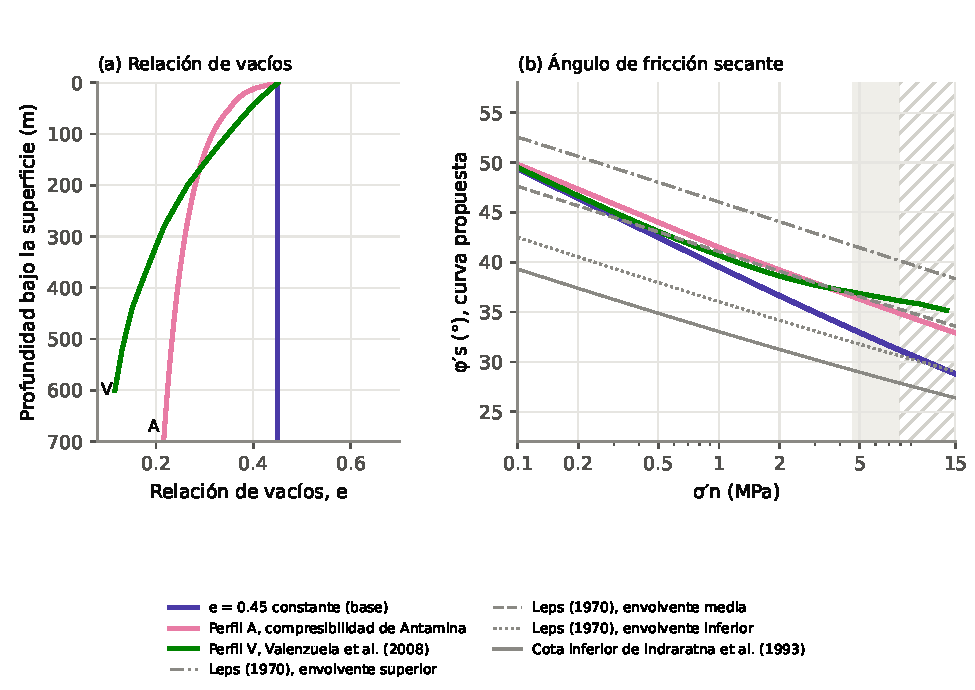
\includegraphics[width=\linewidth]{figs/Fig3_perfil_e.pdf}
\caption{(a) Relación de vacíos con la profundidad: valores constantes y perfiles con densificación desde $e = 0.45$ (A, compresibilidad del edómetro de Antamina; V, forma de la envolvente propuesta por \citealp{valenzuela2008}). (b) Ángulo de fricción secante de la curva propuesta con cada supuesto; zona gris y rayado como en la Fig.~\ref{fig:phi}.}\label{fig:e}\end{figure}

\needspace{10\baselineskip}\section{Sensibilidades y vacíos}\label{sec:vacios}
\begin{itemize}
\item \textbf{Litologías.} Con $m = 0.85$, el $\phi'_1$ medio a $e = 0.45$ es 36.1° en mármol, 39.1° en intrusivo y 42.7° en hornfels. La curva trata el desmonte como un solo material, como el diseño del DDE; donde el volteo concentre mármol, la litología ensayada más débil, la resistencia sería menor: de los 9 ensayos de mármol, 7 quedan bajo la curva propuesta. El mármol descansa en un solo set triaxial de gran escala, con 3 de sus 5 ensayos con ciclos de carga y descarga, en un set de 6~in y en el corte directo de la ruma de mármol ROM de \citet{anddes2024}, y tiene desgaste Los Ángeles de 41--44~\% (nota de \citealp{g2012}), lo que sugiere susceptibilidad a la rotura.
\item \textbf{Condiciones no cubiertas.} La curva es drenada y de máximo desviador. No cubre presiones de poros en capas basales saturadas, colapso por humedecimiento, degradación en el tiempo, condición sísmica ni post-sísmica.
\end{itemize}

\needspace{10\baselineskip}\subsection{Efecto del tamaño de partícula}\label{sec:tamano}
Leps 2.0 no tiene un término de tamaño: en su base mundial, el tamaño medio de partícula ($D_{50}$) no mostró una correlación fuerte con la resistencia, y sus efectos pueden haber quedado bajo el ruido de los datos \citep[Tabla~4]{cylwik}. Los dos pares de escala de Antamina tampoco permiten estimarlo (sección~\ref{sec:metodo}). La teoría de \citet{frossard2012}, en cambio, predice que un material más grueso de la misma roca resiste menos, porque las partículas grandes rompen con menor esfuerzo. Para gradaciones paralelas, la envolvente del material grueso es la del fino con los esfuerzos escalados por $\lambda = (D_{lab}/D_{campo})^{3/m_w}$, donde $m_w$ es el módulo de Weibull de la resistencia de las partículas. Con la envolvente de Leps 2.0, eso equivale a multiplicar $\tau$ por $\lambda^{1-m}$ en todo el rango.

Como no hay ensayos de resistencia de partículas por tamaño en Antamina, Stantec tomó como valor central el exponente de la corrección por tamaño del ensayo de carga puntual, 0.45 \citep{isrm1985}, que equivale a $m_w = 6.7$, y un rango de 4 a 10. Los ensayos del ajuste tienen tres tamaños de partícula: $D_{max} = 178$~mm en los triaxiales de 1~m, 102~mm en los de 0.6~m y 25~mm en las probetas de 6~in y el corte directo. Con $D_{campo} = 1000$~mm, entre la mediana (853~mm) y el percentil 90 (1340~mm) de la fragmentación, resulta la Tabla~\ref{tab:tamano}: con el valor central, $\phi'_1$ bajaría 3.2° si el ensayo representativo es el de 178~mm y 6.7° si es el de 25~mm. \citet{frossard2012} recomiendan limitar la razón de escalamiento a 15: de 178~mm a 1000~mm es 5.6, pero de 25~mm es 39, fuera de ese límite. Los dos pares de escala de Antamina no muestran una diferencia sistemática entre esos tamaños (sección~\ref{sec:metodo}), lo que no es coherente con el efecto teórico entre 25 y 178~mm. El método supone gradaciones paralelas, lo que no se cumple con las gradaciones escalpadas de los ensayos, y no se ha verificado en desmonte de Antamina. Por eso el efecto se informa como sensibilidad y no se aplica a la curva propuesta.

\begin{table}[!htbp]\centering\small\caption{Sensibilidad al tamaño de partícula, del ensayo al desmonte con $D_{campo} = 1000$~mm \citep{frossard2012}: factor sobre $\tau$ y $\phi'_1$ de la curva propuesta a $e = 0.45$.}\label{tab:tamano}
\begin{tabular}{rlrrr}\toprule $D_{lab}$ (mm) & $m_w$ & Factor sobre $\tau$ & $\phi'_1$ (°) & Diferencia (°)\\\midrule
178 & 4.0 & 0.823 & 34.1 & $-$5.3 \\
178 & 6.7 (ISRM) & 0.890 & 36.2 & $-$3.2 \\
178 & 10.0 & 0.925 & 37.3 & $-$2.2 \\
102 & 4.0 & 0.773 & 32.5 & $-$7.0 \\
102 & 6.7 (ISRM) & 0.857 & 35.2 & $-$4.3 \\
102 & 10.0 & 0.902 & 36.6 & $-$2.9 \\
25 & 4.0 & 0.662 & 28.6 & $-$10.9 \\
25 & 6.7 (ISRM) & 0.780 & 32.7 & $-$6.7 \\
25 & 10.0 & 0.848 & 34.9 & $-$4.6 \\
\bottomrule\end{tabular}\end{table}

\subsection*{Riesgos de la curva y cómo se cubren}
La Tabla~\ref{tab:riesgos} resume qué riesgos se cubren hoy con margen o con la forma de aplicar la curva, y cuáles requieren ensayos.
\begin{table}[!htbp]\centering\small\caption{Riesgos principales de la curva propuesta.}\label{tab:riesgos}
\begin{tabular}{L{5.0cm}L{5.6cm}L{4.6cm}}\toprule Riesgo & Cobertura en esta revisión & Qué lo cierra\\\midrule
$e = 0.45$ no medida (cada 0.05 de $e$ cambia $\phi'_1$ en 1°) & Coherente con el $\gamma$ del DDE y con la literatura (Tabla~\ref{tab:ebase}); alternativas 0.55 y 0.65 y perfiles $e(z)$ & Densidad in situ (ítem~1)\\
Mármol, la litología ensayada más débil: un set triaxial de gran escala (enrocado de presa, 3 de 5 ensayos con carga y descarga), uno de 6~in y un corte directo ROM & Curva de un solo material, como el DDE; no cubre sectores con predominio de mármol & Triaxiales de mármol ROM (ítem~2)\\
19 de 22 triaxiales con contracción volumétrica en el máximo desviador (21 si se cuentan los de signo dudoso) & Del lado conservador: el máximo desviador puede subestimar la resistencia última & Ensayos hasta 25~\% de deformación (ítem~2)\\
Curvatura sobre 4.62~MPa & Hipótesis P10--P90 en la banda; sensibilidad con $m = 0.79$ & Triaxiales a alta presión (ítem~4)\\
Segregación por volteo & No cubierta: curva de un solo material, como el DDE & Modelo de bloques y plan de colocación, si el EoR lo requiere\\
Bajo confinamiento: pocos ensayos y dispersos & Verificación de caras y bancos con 37° & --\\
Efecto del tamaño de partícula & Sensibilidad (Tabla~\ref{tab:tamano}); no aplicado a la curva & Ensayos de resistencia de partículas por tamaño (carga puntual o compresión de partículas)\\
\bottomrule\end{tabular}\end{table}

\needspace{10\baselineskip}\section{Ensayos que más reducirían la incertidumbre}\label{sec:ensayos}
La Tabla~\ref{tab:ensayos} ordena los ensayos por el valor de la información para la curva. Las cantidades son mínimas. El costo, el plazo y el laboratorio quedan \colorbox{yellow}{por confirmar}; para $\sigma'_3$ de 3 a 6~MPa en probetas de 1~m hay que confirmar primero que exista el equipo.

\begin{table}[!htbp]\centering\small\caption{Programa de ensayos propuesto.}\label{tab:ensayos}
\begin{tabular}{L{0.4cm}L{3.0cm}L{6.4cm}L{5.0cm}}\toprule & Ensayo & Cantidad y condiciones & Decisión que informa\\\midrule
1 & Densidad in situ & Al menos 10 ensayos de reemplazo de agua en macrocalicatas en botaderos existentes, bajo la capa compactada por el tránsito o en material de cara volteado, repartidos por litología dominante; conciliación de toneladas transportadas contra volumen topográfico por botadero; registro de densidad en sondajes, donde existan, para la variación con la profundidad & $e$ de colocación (base 0.45) y perfil $e(z)$\\
2 & Triaxiales de mármol ROM & Un set de 4 probetas, diámetro de 1~m, $\sigma'_3$ = 0.5, 1.0, 1.5 y 2.0~MPa, $e \approx 0.6$, hasta 25~\% de deformación axial con medición de volumen & Resistencia de la litología ensayada más débil\\
3 & Edómetro de gran escala & Dos ensayos (mármol ROM y desmonte mezclado), diámetro mínimo de 0.6~m, desde $e \approx 0.65$ hasta $\sigma'_v$ de 5~MPa o el máximo del equipo & Compresibilidad del perfil $e(z)$\\
4 & Triaxiales a alta presión & Un set de 3 probetas de mármol, $\sigma'_3$ = 3, 4.5 y 6~MPa, con el mayor diámetro disponible; solo si un mecanismo lleva el diseño a esos esfuerzos & Curvatura $m$ sobre 4.62~MPa\\
\bottomrule\end{tabular}\end{table}

\needspace{10\baselineskip}\section{Implementación en FLAC2D}\label{sec:flac}
FLAC2D (versión 9.0) no tiene un modelo constitutivo con la envolvente de potencia de Leps 2.0, pero la curva se puede usar con el modelo \texttt{mohr-coulomb}: en cada zona, la cohesión y la fricción se reemplazan por las de la recta tangente a la curva en el punto que corresponde al esfuerzo de la zona. El criterio de falla sigue siendo Mohr--Coulomb; lo que cambia de zona a zona son $c'$ y $\phi'$. Los parámetros elásticos no son parte de esta propuesta.

El procedimiento, que una función FISH aplica a todas las zonas del desmonte, es:
\begin{enumerate}
\item Con el $\sigma'_3$ de la zona, $-(\texttt{zone.stress.max} + \texttt{zone.pp})$ porque FLAC usa compresión negativa, se busca el $\sigma'_n$ del punto de tangencia del círculo de falla con la envolvente. Es el mismo cálculo con que este memorándum convierte los triaxiales (Ecs.~10--12 de \citealp{cylwik}).
\item En ese punto, $\tan\phi'_t = m\,\tau/\sigma'_n$ y $c'_t = (1-m)\,\tau$, que se asignan como \texttt{friction} (°) y \texttt{cohesion} (Pa).
\item Como la tangente depende del esfuerzo, la actualización y \texttt{model solve} se alternan hasta que las propiedades dejen de cambiar. Un piso de $\sigma'_3$ (10~kPa) evita que la cohesión se anule en la superficie.
\end{enumerate}
La Tabla~\ref{tab:flac} da los valores tangentes de la curva propuesta ($e = 0.45$) a varios $\sigma'_3$, para comprobar la implementación. La curva es cóncava, así que la recta tangente queda por encima de ella lejos del punto de tangencia: si los esfuerzos cambian después de la última actualización, la resistencia queda sobrestimada. Por eso la actualización se repite hasta converger. El procedimiento admite $e$ variable con la profundidad: basta guardar la $e$ de cada zona en una variable extra (\texttt{zone.extra}) y usarla en $\phi'_1$.

\begin{table}[!htbp]\centering\small\caption{Mohr--Coulomb tangente a la curva propuesta ($e = 0.45$) según el esfuerzo principal menor de la zona, para verificar la implementación en FLAC2D.}\label{tab:flac}
\begin{tabular}{rrrrrr}\toprule $\sigma'_3$ (MPa) & $\sigma'_n$ (MPa) & $\tau$ (kPa) & $\phi'_t$ (°) & $c'_t$ (kPa) & $\sigma'_1 - \sigma'_3$ (MPa)\\\midrule
0.1 & 0.189 & 200.4 & 42.0 & 30.1 & 0.539 \\
0.5 & 0.881 & 740.9 & 35.6 & 111.1 & 1.822 \\
1.0 & 1.707 & 1299.9 & 32.9 & 195.0 & 3.097 \\
2.0 & 3.306 & 2280.0 & 30.4 & 342.0 & 5.286 \\
5.0 & 7.926 & 4793.7 & 27.2 & 719.0 & 10.780 \\
\bottomrule\end{tabular}\end{table}

{\sloppy La librería \texttt{leps2\_tangente.fis}, que acompaña este memorándum, implementa los tres pasos. Se carga con \texttt{program call} después de asignar \texttt{mohr-coulomb} al grupo \texttt{desmonte}; en cada etapa, la función \texttt{leps\_equilibrar} reemplaza al \texttt{model solve}:\par}
{\footnotesize
\begin{verbatim}
fish define leps_tangente
    ; friction (grados) y cohesion (Pa) tangentes en cada zona del grupo
    local phi1 = (leps_pe0 - leps_omega * leps_e) * math.degrad
    local a = math.tan(phi1) * leps_s0 ^ (1.0 - leps_m) / leps_fos
    local s3 = 0.0
    local lo = 0.0
    local hi = 0.0
    local mid = 0.0
    local sn = 0.0
    local t = 0.0
    local beta = 0.0
    local tanphi = 0.0
    local n = 0
    loop foreach local z zone.list
        if zone.isgroup(z, leps_grupo) then
            s3 = math.max(-(zone.stress.max(z) + zone.pp(z)), leps_s3min)
            lo = math.ln(s3)
            hi = math.ln(40.0 * s3)
            loop local k (1, 60)
                mid = 0.5 * (lo + hi)
                sn = math.exp(mid)
                t = a * sn ^ leps_m
                beta = 0.5 * math.atan(leps_m * t / sn) + 0.25 * math.pi
                if sn - t / math.tan(beta) - s3 > 0.0 then
                    hi = mid
                else
                    lo = mid
                endif
            endloop
            sn = math.exp(0.5 * (lo + hi))
            t = a * sn ^ leps_m
            tanphi = leps_m * t / sn
            zone.prop(z, 'friction') = math.atan(tanphi) / math.degrad
            zone.prop(z, 'cohesion') = (1.0 - leps_m) * t
            n = n + 1
        endif
    endloop
    io.out('leps_tangente: ' + string(n) + ' zonas, fos = ' + string(leps_fos))
end

fish define leps_equilibrar(n_vueltas)
    ; actualiza las tangentes y resuelve, n_vueltas veces
    loop local i (1, n_vueltas)
        leps_tangente
        command
            model solve ratio 1e-5 cycles 20000
        endcommand
    endloop
end
\end{verbatim}}

\noindent\textbf{Factor de seguridad.} \texttt{model factor-of-safety} reduce $c'$ y $\tan\phi'$ de cada zona por el mismo factor, lo que equivale a dividir la curva por ese factor en el punto de tangencia, pero deja fijas las tangentes mientras la reducción redistribuye los esfuerzos. Sirve como primera estimación. El valor consistente con la curva se obtiene con una reducción propia: para un factor de prueba $F$ se divide la curva por $F$ (variable \texttt{leps\_fos}), se repiten la actualización y el equilibrio desde el mismo estado guardado (\texttt{model save} y \texttt{model restore}), y se busca por bisección el $F$ con que el modelo deja de converger. En pruebas de Stantec con FLAC2D 9.0, \texttt{model factor-of-safety} no terminó en un talud de arena con cohesión nula; el piso de $\sigma'_3$ deja una cohesión tangente pequeña en la superficie, pero conviene verificar que el cálculo termine.

Antes de usar los resultados se recomienda:
\begin{enumerate}
\item Simular en FLAC triaxiales de una zona a los $\sigma'_3$ de la Tabla~\ref{tab:flac} y comparar el desviador; la diferencia debería ser de pocos por ciento.
\item Leer las propiedades asignadas (\texttt{zone.prop}) en algunas zonas y compararlas con la Tabla~\ref{tab:flac}.
\item Comparar el factor de seguridad de un caso simple con el de un programa de equilibrio límite (por ejemplo, Slide2 con Morgenstern--Price), con la misma geometría y la misma curva, y repetir con la malla de la mitad del tamaño.
\end{enumerate}
La librería pasa la revisión estática de sintaxis de FLAC2D 9.0, pero no se ha corrido en FLAC.

\needspace{10\baselineskip}\section{Limitaciones y uso de este documento}\label{sec:uso}
Este memorándum es un borrador técnico para la revisión del Ingeniero de Registro (EoR) de los botaderos de Antamina, y la curva es una propuesta para esa revisión. La curva propuesta se basa en 37 ensayos de 13 sets, incluidas las dos mezclas, en el criterio Leps 2.0 y en supuestos declarados en el texto ($m$ de la base mundial, $e = 0.45$ y desmonte tratado como un solo material). Su aplicación a un diseño específico requiere la verificación del EoR con los datos del sitio, la geometría, las condiciones de agua y sismo y los criterios de aceptación que correspondan. El documento no incluye análisis de estabilidad.

Stantec usó los resultados de laboratorio de los informes de terceros listados en las referencias (Golder Associates, WSP, IDIEM y Anddes Geolab) tal como fueron informados. Stantec verificó que los valores de la base de datos coincidan con las hojas de laboratorio de cada informe o, donde no hay hoja, con sus gráficos, pero no repitió ni validó los ensayos. Los valores recalculados o leídos de gráficos se indican en el texto y en las notas de las tablas; entre ellos, la $e_0$ y el $B_g$ de \citet{g2012}, la $e$ de los ensayos de \citet{anddes2024} y de \citet{i2025}, las $e_0$ de los edómetros y los $\sigma'_n$ y $\phi'_s$ de los triaxiales, convertidos con Leps 2.0. Stantec preparó esta propuesta con la habilidad y diligencia razonables para el alcance descrito; su uso fuera de ese alcance y de las condiciones aquí descritas es responsabilidad de quien la aplique.

\vspace{6pt}\noindent\begin{tabular}{@{}lll@{}}
Preparado por: & \colorbox{yellow}{XX} & Stantec\\
Revisado por: & \colorbox{yellow}{XX} & Stantec\\
Aprobado por: & \colorbox{yellow}{XX} & Stantec\\
\end{tabular}

\begin{thebibliography}{20}\small
\bibitem[Anddes Geolab(2024)]{anddes2024} Anddes Geolab (2024). \emph{Ensayos de laboratorio en desmonte (rumas M-1 a M-13, H-1 a H-12, I-1 a I-12 y pilas 01 y 02): triaxial CU de 6~in, corte directo de gran escala, clasificación SUCS, Proctor estándar y contenido de agua} [informes de ensayo para Compañía Minera Antamina; solicitud EPE-23.10.141].
\bibitem[Compañía Minera Antamina(2025)]{antamina2025frag} Compañía Minera Antamina (2025). \emph{Fragmentación del desmonte 2025} [base de datos de análisis de fotos post-voladura].
\bibitem[Cylwik et al.(2025)]{cylwik} Cylwik, S.~D., Arrieta, M., Cunning, J.~C., y Hawley, P.~M. (2025). Update to the Leps strength envelopes for rockfill based on 900 large-scale triaxial tests. \emph{International Journal of Geomechanics}, 25(12), 04025285. \url{https://doi.org/10.1061/IJGNAI.GMENG-12050}
\bibitem[Frossard et al.(2012)]{frossard2012} Frossard, E., Hu, W., Dano, C., y Hicher, P.-Y. (2012). Rockfill shear strength evaluation: A rational method based on size effects. \emph{Géotechnique}, 62(5), 415--427. \url{https://doi.org/10.1680/geot.10.P.079}
\bibitem[Golder Associates Perú(2010)]{g2010} Golder Associates Perú (2010). \emph{Caracterización material de ROM -- Proyecto IPCC} [Memorando técnico para Compañía Minera Antamina, proyecto 099-4151017, 25 de marzo de 2010].
\bibitem[Golder Associates Perú(2012)]{g2012} Golder Associates Perú (2012). \emph{Summary of results from laboratory testing program for black marble rockfill} [Technical memorandum Doc.~No.~446, proyectos 1014270482C/1194155017P, 7 de febrero de 2012; anexo IDIEM, Informe 708.397-A].
\bibitem[Golder Associates Perú(2021)]{g2021} Golder Associates Perú (2021). \emph{Estudio conceptual almacenamiento eco-estable de desmonte y relaves: Informe de interpretación de ensayos de laboratorio} [Informe 101-20110-LTE01220-INF-420-G-0013, Rev.~0, 28 de abril de 2021].
\bibitem[Golder Associates Perú(2022)]{w2022} Golder Associates Perú (2022). \emph{Pruebas de enrocado 3B a gran escala material tipo hornfels y de alta presión para el modelamiento de deformación} [Memorando técnico 105-18028-MTE00420-MEM-430-G-0007, 8 de septiembre de 2022; anexos IDIEM, Informes 1.555.677-A a~E].
\bibitem[Hawley y Cunning(2017)]{hc2017} Hawley, P.~M., y Cunning, J. (Eds.). (2017). \emph{Guidelines for mine waste dump and stockpile design}. CSIRO Publishing.
\bibitem[IDIEM(2025)]{i2025} IDIEM (2025). \emph{Ensayos triaxiales a gran escala -- Fase 2 y 3} [Informe de Ensayo Especial 1.966.314-B, Rev.~01, 24 de enero de 2025, para WSP Perú y Compañía Minera Antamina].
\bibitem[Indraratna et al.(1993)]{indraratna1993} Indraratna, B., Wijewardena, L.~S.~S., y Balasubramaniam, A.~S. (1993). Large-scale triaxial testing of greywacke rockfill. \emph{Géotechnique}, 43(1), 37--51. \url{https://doi.org/10.1680/geot.1993.43.1.37}
\bibitem[ISRM(1985)]{isrm1985} International Society for Rock Mechanics. (1985). Suggested method for determining point load strength. \emph{International Journal of Rock Mechanics and Mining Sciences \& Geomechanics Abstracts}, 22(2), 51--60.
\bibitem[Leps(1970)]{leps} Leps, T.~M. (1970). Review of shearing strength of rockfill. \emph{Journal of the Soil Mechanics and Foundations Division}, 96(SM4), 1159--1170.
\bibitem[Marsal(1967)]{marsal1967} Marsal, R.~J. (1967). Large scale testing of rockfill materials. \emph{Journal of the Soil Mechanics and Foundations Division}, 93(SM2), 27--43.
\bibitem[Ovalle et al.(2023)]{ovalle2023} Ovalle, C., Girumugisha, G., Cantor, D., y Ouellet, S. (2023). Size effects assessment of mine waste-rock shear strength combining numerical, laboratory and in situ approaches. En P.~M. Dight (Ed.), \emph{SSIM 2023} (pp.~291--300). Australian Centre for Geomechanics. \url{https://doi.org/10.36487/ACG_repo/2335_16}
\bibitem[Stantec(2023)]{stantec2023} Stantec (2023). \emph{Láminas A.5.4 y A.5.5: propiedades del desmonte chancado y ROM} [láminas de interpretación para Compañía Minera Antamina].
\bibitem[Stantec(2025)]{stantec2025sda} Stantec (2025). \emph{Seismic deformation analysis report: 24213EXB-115 Depósito de Desmonte Este, extensiones E1, E2, E9 y E10} [Informe 102-24213-CW18321-INF-115-R-0005, Rev.~B, 31 de octubre de 2025, para Compañía Minera Antamina].
\bibitem[Stantec(2026a)]{stantec2026dde} Stantec (2026a). \emph{Informe de diseño geotécnico: 24213EXB-115 Depósito de Desmonte Este, extensiones E1, E2, E9 y E10} [Informe 102-24213-CW18321-INF-115-R-0004, Rev.~0, 13 de febrero de 2026, para Compañía Minera Antamina].
\bibitem[Stantec(2026b)]{stantec2026iff} Stantec (2026b). \emph{Informe final de estudio: Depósito de Desmonte Este (DDE), Life Extension 2 Program, ingeniería de prefactibilidad Gate 2B} [Informe 102-24213-CW18321-IFF-115-G-0001, Rev.~B, 6 de abril de 2026, para Compañía Minera Antamina].
\bibitem[Valenzuela et al.(2008)]{valenzuela2008} Valenzuela, L., Bard, E., Campaña, J., y Anabalón, M.~E. (2008). High waste rock dumps: Challenges and developments. En A.~B. Fourie (Ed.), \emph{Rock Dumps 2008: Proceedings of the First International Seminar on the Management of Rock Dumps, Stockpiles and Heap Leach Pads} (pp.~65--78). Australian Centre for Geomechanics. \url{https://doi.org/10.36487/ACG_repo/802_6}
\bibitem[WSP Perú(2023)]{wsp2023tsf} WSP Perú (2023). \emph{Ingeniería de detalle para recrecimiento de depósito de relaves a la cota 4165 m, Presa de Relaves Antamina: Informe final} [Informe 104-22155-MTE00420-IFF-430-G-0001, Rev.~0, 28 de diciembre de 2023, para Compañía Minera Antamina].
\bibitem[WSP Perú(2024)]{w2024} WSP Perú (2024). \emph{Ensayos geotécnicos a gran escala para mezclas de co-disposición de desmonte y relave} [Informe final 101-20110-LTE01220-IFF-420-G-0003, Fase~1, 30 de octubre de 2024; anexos IDIEM 1.914.482-A a~G].
\end{thebibliography}

\clearpage
\appendix
\renewcommand{\thetable}{A\arabic{table}}\setcounter{table}{0}
\section{Ensayos de resistencia disponibles y su uso}\label{sec:anexo}
La Tabla~\ref{tab:anx_todos} da, ensayo por ensayo, los 120 ensayos de resistencia de desmonte de la Tabla~\ref{tab:inventario}, agrupados por su uso en este memorándum: 37 en el ajuste de la curva propuesta (incluidas las dos mezclas), 36 de contraste y 47 no usados, con el motivo. Los esfuerzos son efectivos, en la falla: en los triaxiales drenados, en el máximo desviador; en los no drenados, en la máxima oblicuidad o, donde el informe no lo permite \citep{g2010}, en el máximo desviador; en el corte directo, $\tau$ pico y $\sigma'_n$ medidos. En los triaxiales, $\sigma'_n$ y $\phi'_s$ se calcularon con la conversión de Leps 2.0 con $m = 0.85$, como en la Tabla~\ref{tab:datos}, y $\phi'_s$ está a la $e_0$ de cada ensayo, sin corregir por densidad. Los edómetros están en la Tabla~\ref{tab:edo}.

\begin{footnotesize}\setlength{\tabcolsep}{2.5pt}
\begin{longtable}{L{3.6cm}L{2.2cm}rrrrrrrr}
\caption{Ensayos de resistencia de desmonte de Antamina y su uso. $D$: diámetro de la probeta o lado de la caja; $D_{max}$: tamaño máximo de partícula (--: no informado); $\varepsilon_a$: deformación axial en la falla.}\label{tab:anx_todos}\\
\toprule Set & Litología & $D$ & $D_{max}$ & $e_0$ & $\sigma'_3$ & $\sigma'_1$ & $\sigma'_n$ & $\phi'_s$ & $\varepsilon_a$\\
 & & (m) & (mm) & & (MPa) & (MPa) & (MPa) & (°) & (\%)\\\endfirsthead
\toprule Set & Litología & $D$ & $D_{max}$ & $e_0$ & $\sigma'_3$ & $\sigma'_1$ & $\sigma'_n$ & $\phi'_s$ & $\varepsilon_a$\\\midrule\endhead
\midrule\multicolumn{10}{p{14.2cm}}{\textbf{Ajuste de la curva propuesta}} \\
\multicolumn{10}{p{14.2cm}}{\textit{\citet{g2012}, triaxial CD}} \\
G2012-MN-C & mármol & 1.00 & 178 & 0.312 & 0.49 & 2.27 & 0.86 & 40.0 & 17.3 \\
G2012-MN-C & mármol & 1.00 & 178 & 0.312 & 0.49 & 2.19 & 0.86 & 39.2 & 18.3 \\
G2012-MN-C & mármol & 1.00 & 178 & 0.312 & 0.98 & 3.90 & 1.66 & 36.6 & 18.0 \\
G2012-MN-C & mármol & 1.00 & 178 & 0.312 & 1.96 & 7.78 & 3.32 & 36.6 & 19.6 \\
G2012-MN-C & mármol & 1.00 & 178 & 0.312 & 1.96 & 8.29 & 3.38 & 38.0 & 17.8 \\
\multicolumn{10}{p{14.2cm}}{\textit{\citet{g2021}, triaxial CD}} \\
G21-DESM-COMP & compuesto & 0.15 & 25 & 0.322 & 0.10 & 0.38 & 0.16 & 36.1 & 4.0 \\
G21-DESM-COMP & compuesto & 0.15 & 25 & 0.322 & 0.40 & 1.92 & 0.71 & 40.8 & 20.2 \\
G21-DESM-COMP & compuesto & 0.15 & 25 & 0.324 & 1.20 & 5.85 & 2.14 & 41.1 & 12.1 \\
\multicolumn{10}{p{14.2cm}}{\textit{\citet{w2022}, triaxial CD}} \\
HF-1.0m-IDIEM-mono & hornfels & 1.00 & 178 & 0.332 & 0.98 & 4.88 & 1.76 & 41.5 & 13.1 \\
HF-1.0m-IDIEM-mono & hornfels & 1.00 & 178 & 0.332 & 1.96 & 11.02 & 3.61 & 44.1 & 19.0 \\
HF-1.0m-IDIEM-mono & hornfels & 1.00 & 178 & 0.332 & 2.45 & 14.38 & 4.56 & 44.9 & 17.8 \\
HF-1.0m-IDIEM-cd & hornfels & 1.00 & 178 & 0.357 & 0.98 & 4.80 & 1.75 & 41.2 & 19.1 \\
HF-1.0m-IDIEM-cd & hornfels & 1.00 & 178 & 0.357 & 1.96 & 11.66 & 3.66 & 45.2 & 18.8 \\
HF-1.0m-IDIEM-cd & hornfels & 1.00 & 178 & 0.357 & 2.45 & 15.38 & 4.62 & 46.3 & 19.0 \\
HF-0.15m-Golder & hornfels & 0.15 & 25 & 0.333 & 0.98 & 5.08 & 1.77 & 42.5 & 11.4 \\
MN-0.15m-Golder & mármol & 0.15 & 25 & 0.327 & 0.98 & 4.80 & 1.75 & 41.2 & 18.5 \\
\multicolumn{10}{p{14.2cm}}{\textit{\citet{w2024}, triaxial CD}} \\
WSP24\_C4\_MON & intrusivo & 0.60 & 102 & 0.354 & 0.49 & 2.13 & 0.85 & 38.6 & 12.4 \\
WSP24\_C4\_MON & intrusivo & 0.60 & 102 & 0.354 & 0.98 & 4.37 & 1.71 & 39.2 & 20.7 \\
WSP24\_C4\_MON & intrusivo & 0.60 & 102 & 0.354 & 1.96 & 8.98 & 3.45 & 39.8 & 19.4 \\
\multicolumn{10}{p{14.2cm}}{\textit{\citet{i2025}, triaxial CD}} \\
Intrusivo 100 ~\% & intrusivo & 1.00 & 178 & 0.290 & 0.49 & 2.17 & 0.85 & 39.0 & 4.0 \\
Intrusivo 100 ~\% & intrusivo & 1.00 & 178 & 0.290 & 0.98 & 4.43 & 1.72 & 39.5 & 13.0 \\
Intrusivo 100 ~\% & intrusivo & 1.00 & 178 & 0.290 & 1.96 & 8.69 & 3.42 & 39.0 & 11.2 \\
\multicolumn{10}{p{14.2cm}}{\textit{\citet{anddes2024}, corte directo}} \\
Ruma 02 & hornfels & 0.31 & 25 & 0.332 & -- & -- & 0.30 & 40.4 & -- \\
Ruma 02 & hornfels & 0.31 & 25 & 0.332 & -- & -- & 0.60 & 38.4 & -- \\
Ruma 02 & hornfels & 0.31 & 25 & 0.332 & -- & -- & 1.20 & 39.8 & -- \\
Ruma 03 / Fase 10 A & intrusivo & 0.31 & 25 & 0.410 & -- & -- & 0.30 & 37.2 & -- \\
Ruma 03 / Fase 10 A & intrusivo & 0.31 & 25 & 0.410 & -- & -- & 0.60 & 38.0 & -- \\
Ruma 03 / Fase 10 A & intrusivo & 0.31 & 25 & 0.410 & -- & -- & 1.20 & 38.2 & -- \\
Ruma 01 & mármol & 0.31 & 25 & 0.262 & -- & -- & 0.30 & 36.2 & -- \\
Ruma 01 & mármol & 0.31 & 25 & 0.262 & -- & -- & 0.60 & 38.0 & -- \\
Ruma 01 & mármol & 0.31 & 25 & 0.262 & -- & -- & 1.20 & 39.4 & -- \\
Pila 01 (Mármol + Hornfels) & mármol--hornfels & 0.31 & 25 & 0.326 & -- & -- & 0.30 & 49.9 & -- \\
Pila 01 (Mármol + Hornfels) & mármol--hornfels & 0.31 & 25 & 0.326 & -- & -- & 0.60 & 46.2 & -- \\
Pila 01 (Mármol + Hornfels) & mármol--hornfels & 0.31 & 25 & 0.326 & -- & -- & 1.00 & 43.4 & -- \\
Pila 02 (Intrusivo) & intrusivo & 0.31 & 25 & 0.479 & -- & -- & 0.30 & 49.7 & -- \\
Pila 02 (Intrusivo) & intrusivo & 0.31 & 25 & 0.479 & -- & -- & 0.60 & 46.6 & -- \\
Pila 02 (Intrusivo) & intrusivo & 0.31 & 25 & 0.479 & -- & -- & 1.20 & 40.3 & -- \\
\midrule\multicolumn{10}{p{14.2cm}}{\textbf{Contraste (sección~\ref{sec:contraste})}} \\
\multicolumn{10}{p{14.2cm}}{\textit{\citet{anddes2024}, triaxial CU: triaxial no drenado (CU), máxima oblicuidad}} \\
Ruma 01 (M-1 al M-13) & mármol & 0.15 & -- & 0.263 & 0.08 & 0.45 & 0.15 & 44.5 & 15.0 \\
Ruma 01 (M-1 al M-13) & mármol & 0.15 & -- & 0.263 & 0.11 & 1.00 & 0.22 & 53.6 & 15.0 \\
Ruma 01 (M-1 al M-13) & mármol & 0.15 & -- & 0.263 & 0.42 & 2.44 & 0.78 & 44.8 & 15.0 \\
Ruma 02 (H-1 al H-12) & hornfels & 0.15 & -- & 0.332 & 0.07 & 0.63 & 0.14 & 52.4 & 15.0 \\
Ruma 02 (H-1 al H-12) & hornfels & 0.15 & -- & 0.332 & 0.09 & 1.08 & 0.20 & 56.7 & 15.0 \\
Ruma 02 (H-1 al H-12) & hornfels & 0.15 & -- & 0.332 & 0.31 & 1.90 & 0.58 & 45.7 & 15.0 \\
Ruma 03 / Fase 10 A (I-1 al I-12) & intrusivo & 0.15 & -- & 0.410 & 0.12 & 0.84 & 0.24 & 48.0 & 15.0 \\
Ruma 03 / Fase 10 A (I-1 al I-12) & intrusivo & 0.15 & -- & 0.410 & 0.13 & 1.12 & 0.26 & 51.8 & 15.0 \\
Ruma 03 / Fase 10 A (I-1 al I-12) & intrusivo & 0.15 & -- & 0.410 & 0.29 & 1.97 & 0.55 & 48.0 & 15.0 \\
Pila 01 (MP1-B-M-1, MP1-B-M2, MP1-B-M3, MP1-H-Material B) & mármol--hornfels & 0.15 & -- & 0.326 & 0.10 & 0.68 & 0.19 & 48.2 & 15.0 \\
Pila 01 (MP1-B-M-1, MP1-B-M2, MP1-B-M3, MP1-H-Material B) & mármol--hornfels & 0.15 & -- & 0.326 & 0.20 & 1.41 & 0.38 & 48.7 & 15.0 \\
Pila 01 (MP1-B-M-1, MP1-B-M2, MP1-B-M3, MP1-H-Material B) & mármol--hornfels & 0.15 & -- & 0.326 & 0.69 & 3.75 & 1.26 & 43.5 & 15.0 \\
Pila 02 (MP2-A-M-1 a MP2-A-M-5, MP2-H-Material A) & intrusivo & 0.15 & -- & 0.479 & 0.11 & 0.71 & 0.21 & 46.2 & 15.0 \\
Pila 02 (MP2-A-M-1 a MP2-A-M-5, MP2-H-Material A) & intrusivo & 0.15 & -- & 0.479 & 0.23 & 1.60 & 0.44 & 48.3 & 15.0 \\
Pila 02 (MP2-A-M-1 a MP2-A-M-5, MP2-H-Material A) & intrusivo & 0.15 & -- & 0.479 & 0.63 & 3.42 & 1.16 & 43.2 & 15.0 \\
\multicolumn{10}{p{14.2cm}}{\textit{\citet{g2010}, triaxial CU: triaxial no drenado (CU), máximo desviador}} \\
G2010-A-MN-2.8in & mármol & 0.07 & 10 & 0.290 & 0.62 & 2.84 & 1.09 & 39.8 & 8.3 \\
G2010-A-MN-2.8in & mármol & 0.07 & 10 & 0.295 & 0.72 & 3.11 & 1.24 & 38.6 & 7.6 \\
G2010-A-MN-2.8in & mármol & 0.07 & 10 & 0.290 & 0.87 & 3.61 & 1.49 & 37.6 & 5.3 \\
G2010-A-HG-2.8in & hornfels & 0.07 & 10 & 0.377 & 0.22 & 0.92 & 0.37 & 38.2 & 1.9 \\
G2010-A-HG-2.8in & hornfels & 0.07 & 10 & 0.377 & 0.30 & 1.21 & 0.51 & 36.7 & 1.8 \\
G2010-A-HG-2.8in & hornfels & 0.07 & 10 & 0.377 & 0.54 & 2.07 & 0.90 & 36.0 & 2.5 \\
G2010-A-INT-2.8in & intrusivo & 0.07 & 10 & 0.434 & 0.26 & 1.13 & 0.45 & 38.5 & 1.6 \\
G2010-A-INT-2.8in & intrusivo & 0.07 & 10 & 0.434 & 0.39 & 1.58 & 0.67 & 36.8 & 1.9 \\
G2010-A-INT-2.8in & intrusivo & 0.07 & 10 & 0.434 & 0.53 & 1.93 & 0.87 & 34.7 & 1.7 \\
G2010-A-EXO-2.8in & skarn & 0.07 & 10 & 0.532 & 0.19 & 0.56 & 0.30 & 29.3 & 1.1 \\
G2010-A-EXO-2.8in & skarn & 0.07 & 10 & 0.531 & 0.32 & 0.88 & 0.48 & 28.1 & 1.2 \\
G2010-A-EXO-2.8in & skarn & 0.07 & 10 & 0.532 & 0.49 & 1.41 & 0.75 & 29.1 & 1.3 \\
G2010-A-HG-4in & hornfels & 0.10 & 16 & 0.377 & 0.22 & 1.05 & 0.40 & 40.2 & 1.0 \\
G2010-A-HG-4in & hornfels & 0.10 & 16 & 0.381 & 0.24 & 1.09 & 0.42 & 39.3 & 0.8 \\
G2010-A-HG-4in & hornfels & 0.10 & 16 & 0.377 & 0.40 & 1.34 & 0.65 & 32.5 & 1.0 \\
G2010-A-INT-4in & intrusivo & 0.10 & 16 & 0.435 & 0.10 & 0.37 & 0.16 & 35.0 & 1.4 \\
G2010-A-INT-4in & intrusivo & 0.10 & 16 & 0.435 & 0.17 & 0.66 & 0.28 & 36.6 & 2.2 \\
G2010-A-INT-4in & intrusivo & 0.10 & 16 & 0.435 & 0.18 & 0.83 & 0.32 & 39.5 & 14.6 \\
G2010-A-EXO-4in & skarn & 0.10 & 16 & 0.598 & 0.16 & 0.51 & 0.25 & 32.1 & 1.4 \\
G2010-A-EXO-4in & skarn & 0.10 & 16 & 0.695 & 0.23 & 0.66 & 0.36 & 28.7 & 1.7 \\
G2010-A-EXO-4in & skarn & 0.10 & 16 & 0.703 & 0.36 & 1.02 & 0.55 & 28.6 & 1.2 \\
\midrule\multicolumn{10}{p{14.2cm}}{\textbf{No usado}} \\
\multicolumn{10}{p{14.2cm}}{\textit{\citet{w2022}, triaxial cíclico y monótono: carga cíclica (compresión y extensión) previa a la carga monótona}} \\
HF-USC-ciclico-350 & hornfels & 0.15 & 25 & 0.239 & 0.35 & 1.77 & 0.63 & 41.9 & 20.0 \\
HF-USC-ciclico-350 & hornfels & 0.10 & 25 & 0.239 & 0.35 & 1.63 & 0.62 & 40.1 & 1.7 \\
HF-USC-ciclico-350 & hornfels & 0.10 & 25 & 0.239 & 0.35 & 1.56 & 0.61 & 39.2 & 7.4 \\
MN-USC-ciclico-350 & mármol & 0.10 & 25 & 0.205 & 0.35 & 1.60 & 0.61 & 39.7 & 4.9 \\
MN-USC-ciclico-350 & mármol & 0.15 & 25 & 0.205 & 0.35 & 1.93 & 0.64 & 43.6 & -- \\
MN-USC-ciclico-350 & mármol & 0.15 & 25 & 0.205 & 0.35 & 1.90 & 0.64 & 43.4 & -- \\
\multicolumn{10}{p{14.2cm}}{\textit{\citet{w2022}, triaxial CD: duplicado de Golder Associates Perú (2012); se usa el original}} \\
MN-1.0m-IDIEM-2011 & mármol & 1.00 & 178 & 0.312 & 0.49 & 2.27 & 0.86 & 40.0 & 17.3 \\
MN-1.0m-IDIEM-2011 & mármol & 1.00 & 178 & 0.312 & 0.49 & 2.19 & 0.86 & 39.2 & 18.3 \\
MN-1.0m-IDIEM-2011 & mármol & 1.00 & 178 & 0.312 & 0.98 & 3.90 & 1.66 & 36.6 & 18.0 \\
MN-1.0m-IDIEM-2011 & mármol & 1.00 & 178 & 0.312 & 1.96 & 7.78 & 3.32 & 36.6 & 19.6 \\
MN-1.0m-IDIEM-2011 & mármol & 1.00 & 178 & 0.312 & 1.96 & 8.29 & 3.38 & 38.0 & 17.8 \\
\multicolumn{10}{p{14.2cm}}{\textit{\citet{g2010}, triaxial CU: material chancado (fase B)}} \\
G2010-B-MN-2.8in & mármol & 0.07 & 10 & 0.278 & 0.71 & 3.49 & 1.28 & 41.1 & 5.8 \\
G2010-B-MN-2.8in & mármol & 0.07 & 10 & 0.273 & 0.82 & 3.73 & 1.44 & 39.5 & 5.1 \\
G2010-B-MN-2.8in & mármol & 0.07 & 10 & 0.273 & 1.03 & 4.62 & 1.80 & 39.3 & 6.3 \\
G2010-B-HG-2.8in & hornfels & 0.07 & 10 & 0.312 & 0.10 & 0.52 & 0.17 & 43.6 & 1.3 \\
G2010-B-HG-2.8in & hornfels & 0.07 & 10 & 0.312 & 0.27 & 1.03 & 0.45 & 35.7 & 1.0 \\
G2010-B-HG-2.8in & hornfels & 0.07 & 10 & 0.311 & 0.40 & 1.90 & 0.71 & 40.5 & 15.2 \\
G2010-B-INT-2.8in & intrusivo & 0.07 & 10 & 0.358 & 0.17 & 0.75 & 0.29 & 39.1 & 1.0 \\
G2010-B-INT-2.8in & intrusivo & 0.07 & 10 & 0.358 & 0.38 & 1.50 & 0.65 & 36.2 & 1.6 \\
G2010-B-INT-2.8in & intrusivo & 0.07 & 10 & 0.358 & 0.49 & 1.90 & 0.83 & 35.8 & 1.5 \\
G2010-B-EXO-2.8in & skarn & 0.07 & 10 & 0.417 & 0.19 & 0.79 & 0.33 & 37.6 & 0.9 \\
G2010-B-EXO-2.8in & skarn & 0.07 & 10 & 0.416 & 0.31 & 1.17 & 0.52 & 35.4 & 1.0 \\
G2010-B-EXO-2.8in & skarn & 0.07 & 10 & 0.416 & 0.51 & 2.02 & 0.86 & 36.7 & 1.5 \\
G2010-B-MN-4in & mármol & 0.10 & 16 & 0.505 & 0.13 & 0.42 & 0.20 & 32.5 & 1.2 \\
G2010-B-MN-4in & mármol & 0.10 & 16 & 0.506 & 0.25 & 0.60 & 0.37 & 23.8 & 0.5 \\
G2010-B-MN-4in & mármol & 0.10 & 16 & 0.595 & 0.35 & 0.82 & 0.50 & 23.7 & 0.5 \\
G2010-B-HG-4in & hornfels & 0.10 & 16 & 0.502 & 0.17 & 0.42 & 0.25 & 24.4 & 0.9 \\
G2010-B-HG-4in & hornfels & 0.10 & 16 & 0.501 & 0.21 & 0.55 & 0.32 & 26.0 & 1.3 \\
G2010-B-HG-4in & hornfels & 0.10 & 16 & 0.503 & 0.46 & 1.05 & 0.65 & 23.0 & 1.0 \\
G2010-B-INT-4in & intrusivo & 0.10 & 16 & 0.492 & 0.18 & 0.43 & 0.27 & 23.4 & 0.6 \\
G2010-B-INT-4in & intrusivo & 0.10 & 16 & 0.498 & 0.25 & 0.55 & 0.36 & 21.6 & 0.6 \\
G2010-B-INT-4in & intrusivo & 0.10 & 16 & 0.492 & 0.33 & 0.78 & 0.47 & 23.9 & 0.6 \\
G2010-B-EXO-4in & skarn & 0.10 & 16 & 0.539 & 0.14 & 0.38 & 0.21 & 28.2 & 1.2 \\
G2010-B-EXO-4in & skarn & 0.10 & 16 & 0.534 & 0.20 & 0.59 & 0.32 & 28.8 & 1.2 \\
G2010-B-EXO-4in & skarn & 0.10 & 16 & 0.538 & 0.31 & 0.82 & 0.46 & 26.9 & 1.2 \\
G2010-B-MN-6in & mármol & 0.15 & 25 & 0.355 & 0.21 & 0.95 & 0.37 & 39.4 & 1.5 \\
G2010-B-MN-6in & mármol & 0.15 & 25 & 0.357 & 0.21 & 0.86 & 0.35 & 37.5 & 1.0 \\
G2010-B-MN-6in & mármol & 0.15 & 25 & 0.357 & 0.06 & 0.35 & 0.12 & 43.4 & 1.0 \\
G2010-B-HG-6in & hornfels & 0.15 & 25 & 0.312 & 0.15 & 0.70 & 0.27 & 39.7 & 1.2 \\
G2010-B-HG-6in & hornfels & 0.15 & 25 & 0.310 & 0.11 & 0.55 & 0.20 & 41.1 & 1.0 \\
G2010-B-HG-6in & hornfels & 0.15 & 25 & 0.310 & 0.05 & 0.24 & 0.09 & 40.7 & 0.5 \\
G2010-B-INT-6in & intrusivo & 0.15 & 25 & 0.353 & 0.09 & 0.39 & 0.16 & 38.0 & 1.8 \\
G2010-B-INT-6in & intrusivo & 0.15 & 25 & 0.354 & 0.03 & 0.13 & 0.06 & 35.6 & 1.2 \\
G2010-B-INT-6in & intrusivo & 0.15 & 25 & 0.355 & 0.03 & 0.08 & 0.05 & 23.4 & 0.8 \\
G2010-B-EXO-6in & skarn & 0.15 & 25 & 0.419 & 0.22 & 1.10 & 0.39 & 41.7 & 1.2 \\
G2010-B-EXO-6in & skarn & 0.15 & 25 & 0.418 & 0.13 & 0.62 & 0.23 & 40.2 & 1.0 \\
G2010-B-EXO-6in & skarn & 0.15 & 25 & 0.431 & 0.11 & 0.55 & 0.20 & 40.9 & 1.0 \\
\bottomrule
\end{longtable}\end{footnotesize}
\end{document}
